%----------------------------------------------------------------------------------------
%	PACKAGES AND OTHER DOCUMENT CONFIGURATIONS
%----------------------------------------------------------------------------------------

\documentclass[nobib]{tufte-book} % Use the tufte-book class which in turn uses the tufte-common class

\usepackage{natbib}

\hypersetup{colorlinks} % Comment this line if you don't wish to have colored links

\usepackage{microtype} % Improves character and word spacing

\usepackage{lipsum} % Inserts dummy text

\usepackage{booktabs} % Better horizontal rules in tables

\usepackage{graphicx} % Needed to insert images into the document
\graphicspath{{graphics/}} % Sets the default location of pictures
\setkeys{Gin}{width=\linewidth,totalheight=\textheight,keepaspectratio} % Improves figure scaling

\usepackage{fancyvrb} % Allows customization of verbatim environments
\fvset{fontsize=\normalsize} % The font size of all verbatim text can be changed here

% \newcommand{\hangp}[1]{\makebox[0pt][r]{(}#1\makebox[0pt][l]{)}} % New command to create parentheses around text in tables which take up no horizontal space - this improves column spacing
% \newcommand{\hangstar}{\makebox[0pt][l]{*}} % New command to create asterisks in tables which take up no horizontal space - this improves column spacing

\usepackage{xspace} % Used for printing a trailing space better than using a tilde (~) using the \xspace command

\usepackage{enumitem} % Used for hypothesis list

\newcommand{\monthyear}{\ifcase\month\or January\or February\or March\or April\or May\or June\or July\or August\or September\or October\or November\or December\fi\space\number\year} % A command to print the current month and year

\newcommand{\openepigraph}[2]{ % This block sets up a command for printing an epigraph with 2 arguments - the quote and the author
\begin{fullwidth}
\sffamily\large
\begin{doublespace}
\noindent\allcaps{#1}\\ % The quote
\noindent\allcaps{#2} % The author
\end{doublespace}
\end{fullwidth}
}

\newcommand{\blankpage}{\newpage\hbox{}\thispagestyle{empty}\newpage} % Command to insert a blank page

\usepackage{units} % Used for printing standard units

\newcommand{\hlred}[1]{\textcolor{Maroon}{#1}} % Print text in maroon
\newcommand{\hangleft}[1]{\makebox[0pt][r]{#1}} % Used for printing commands in the index, moves the slash left so the command name aligns with the rest of the text in the index
\newcommand{\hairsp}{\hspace{1pt}} % Command to print a very short space
\newcommand{\ie}{\textit{i.\hairsp{}e.}\xspace} % Command to print i.e.
\newcommand{\eg}{\textit{e.\hairsp{}g.}\xspace} % Command to print e.g.
\newcommand{\na}{\quad--} % Used in tables for N/A cells
\newcommand{\measure}[3]{#1/#2$\times$\unit[#3]{pc}} % Typesets the font size, leading, and measure in the form of: 10/12x26 pc.
\newcommand{\tuftebs}{\symbol{'134}} % Command to print a backslash in tt type in OT1/T1

\providecommand{\XeLaTeX}{X\lower.5ex\hbox{\kern-0.15em\reflectbox{E}}\kern-0.1em\LaTeX}
\newcommand{\tXeLaTeX}{\XeLaTeX\index{XeLaTeX@\protect\XeLaTeX}} % Command to print the XeLaTeX logo while simultaneously adding the position to the index

\newcommand{\doccmdnoindex}[2][]{\texttt{\tuftebs#2}} % Command to print a command in texttt with a backslash of tt type without inserting the command into the index

\newcommand{\doccmddef}[2][]{\hlred{\texttt{\tuftebs#2}}\label{cmd:#2}\ifthenelse{\isempty{#1}} % Command to define a command in red and add it to the index
{ % If no package is specified, add the command to the index
\index{#2 command@\protect\hangleft{\texttt{\tuftebs}}\texttt{#2}}% Command name
}
{ % If a package is also specified as a second argument, add the command and package to the index
\index{#2 command@\protect\hangleft{\texttt{\tuftebs}}\texttt{#2} (\texttt{#1} package)}% Command name
\index{#1 package@\texttt{#1} package}\index{packages!#1@\texttt{#1}}% Package name
}}

\newcommand{\doccmd}[2][]{% Command to define a command and add it to the index
\texttt{\tuftebs#2}%
\ifthenelse{\isempty{#1}}% If no package is specified, add the command to the index
{%
\index{#2 command@\protect\hangleft{\texttt{\tuftebs}}\texttt{#2}}% Command name
}
{%
\index{#2 command@\protect\hangleft{\texttt{\tuftebs}}\texttt{#2} (\texttt{#1} package)}% Command name
\index{#1 package@\texttt{#1} package}\index{packages!#1@\texttt{#1}}% Package name
}}

% A bunch of new commands to print commands, arguments, environments, classes, etc within the text using the correct formatting
\newcommand{\docopt}[1]{\ensuremath{\langle}\textrm{\textit{#1}}\ensuremath{\rangle}}
\newcommand{\docarg}[1]{\textrm{\textit{#1}}}
\newenvironment{docspec}{\begin{quotation}\ttfamily\parskip0pt\parindent0pt\ignorespaces}{\end{quotation}}
\newcommand{\docenv}[1]{\texttt{#1}\index{#1 environment@\texttt{#1} environment}\index{environments!#1@\texttt{#1}}}
\newcommand{\docenvdef}[1]{\hlred{\texttt{#1}}\label{env:#1}\index{#1 environment@\texttt{#1} environment}\index{environments!#1@\texttt{#1}}}
\newcommand{\docpkg}[1]{\texttt{#1}\index{#1 package@\texttt{#1} package}\index{packages!#1@\texttt{#1}}}
\newcommand{\doccls}[1]{\texttt{#1}}
\newcommand{\docclsopt}[1]{\texttt{#1}\index{#1 class option@\texttt{#1} class option}\index{class options!#1@\texttt{#1}}}
\newcommand{\docclsoptdef}[1]{\hlred{\texttt{#1}}\label{clsopt:#1}\index{#1 class option@\texttt{#1} class option}\index{class options!#1@\texttt{#1}}}
\newcommand{\docmsg}[2]{\bigskip\begin{fullwidth}\noindent\ttfamily#1\end{fullwidth}\medskip\par\noindent#2}
\newcommand{\docfilehook}[2]{\texttt{#1}\index{file hooks!#2}\index{#1@\texttt{#1}}}
\newcommand{\doccounter}[1]{\texttt{#1}\index{#1 counter@\texttt{#1} counter}}

\usepackage{makeidx} % Used to generate the index
\makeindex % Generate the index which is printed at the end of the document

%----------------------------------------------------------------------------------------
%	BOOK META-INFORMATION
%----------------------------------------------------------------------------------------

\title{Design and Evaluation of Spatial Interfaces in Virtual Reality} % Title of the book

\author[Tobias Bernard]{Tobias\ Bernard} % Author

% \supervisors{David Lindlbauer, Prof. Dr. Marc Alex}

\publisher{TU Berlin} % Publisher

%----------------------------------------------------------------------------------------

\begin{document}

\frontmatter

%----------------------------------------------------------------------------------------

\maketitlepage % Print the title page

%----------------------------------------------------------------------------------------
%	COPYRIGHT PAGE
%----------------------------------------------------------------------------------------

\newpage
\begin{fullwidth}
~\vfill
\thispagestyle{empty}
\setlength{\parindent}{0pt}
\setlength{\parskip}{\baselineskip}
Copyright \copyright\ \the\year\ \thanklessauthor

\par This thesis uses the Tufte-Latex template (\url{http://tufte-latex.googlecode.com}) licensed under the Apache License, Version 2.0 (the ``License''); you may not use this file except in compliance with the License. You may obtain a copy of the License at \url{http://www.apache.org/licenses/LICENSE-2.0}. Unless required by applicable law or agreed to in writing, software distributed under the License is distributed on an \smallcaps{``AS IS'' BASIS, WITHOUT WARRANTIES OR CONDITIONS OF ANY KIND}, either express or implied. See the License for the specific language governing permissions and limitations under the License.\index{license}

\end{fullwidth}


\newpage
% \begin{fullwidth}
\setlength{\parindent}{0pt}
\setlength{\parskip}{\baselineskip}

~\vspace{5pc}
\section{Declaration}
\par I hereby declare that I have completed this thesis independently without any unauthorized external help using only the cited sources and references.

~\vspace{3pc}
\section{Deklaration}
\par Hiermit erkl{\"a}re ich, dass ich die vorliegende Arbeit selbstst{\"a}ndig und eigenh{\"a}ndig sowie ohne unerlaubte fremde Hilfe und ausschlie{\ss}lich unter Verwendung der aufgef{\"u}hrten Quellen und Hilfsmittel angefertigt habe.

~\vspace{3pc}

\emph{Berlin, March 2018}

\line(1,0){250}

% \end{fullwidth}


%----------------------------------------------------------------------------------------

\tableofcontents % Print the table of contents


\mainmatter

%----------------------------------------------------------------------------------------
%	ABSTRACT
%----------------------------------------------------------------------------------------

% \cleardoublepage
\chapter{Abstract}
In order to display more information than the screen can accommodate at any one time, graphical user interfaces often clip the content, \ie they employ a virtual space larger than the screen, which users can interactively navigate. Because users can only see a small part of the clipped data space at any given time, it is harder for them to establish a mental model of the data. This can make interfaces difficult to navigate, especially with large amounts of content.

Many Virtual Reality applications today employ the same clipping patterns as traditional 2D interfaces. Our hypothesis is that by using all the possibilities afforded by the 3D environment (such as the user's ability to move and turn their head), \textsc{vr} applications can be made easier to navigate than is the case with clipping-based approaches.

To test this hypothesis we ran a study in which we compared three different interface types: \emph{Spatial} (a grid), \emph{Stacked} (a three-dimensional scrolling list), and \emph{Clipped} (a clipped scrolling list). The content was sets of 20, 50, or 150 square cards with simple icons. We tested all conditions with \emph{Monochrome} and colorful card backgrounds (10 different randomly assigned colors). For each of the 18 resulting conditions, participants were instructed to find a series of icons as quickly as possible.

Participants found the target icons significantly faster in \emph{Spatial} condiitons compared to \emph{Stacked} and \emph{Clipped}. Colorful backgrounds also improved the task performance significantly. We did not find a quantitative difference between \emph{Stacked} and \emph{Clipped}, but in our post-experiment questionnaire users expressed a significant preference for \emph{Stacked}.

\chapter{Zusammenfassung}
Zur Darstellung von gro{\ss}en Informationsmengen, welche nicht gleichzeitig auf den Bildschirm passen, wird in traditionellen grafischen Oberfl{\"a}chen h{\"a}ufig ``clipping'' (ausschneiden, beschneiden) verwendet. Dabei wird der Inhalt auf einer Fl{\"a}che dargestellt, welche gr{\"o}{\ss}er als der Bildschirm ist. Der sichtbare Ausschnitt des Bildes kann von Nutzern interaktiv verschoben werden. Da immer ein Teil des Inhalts sichtbar ist, f{\"a}llt es Nutzern schwer, sich ein mentales Modell der Daten zu bilden, was die Navigation schwieriger machen kann.

Viele Virtual Reality Anwendungen verwenden dieselben ``clipping'' Patterns wie traditionelle 2D Oberfl{\"a}chen. Unsere Hypothese ist, dass durch die Nutzung des vollen Potentials der dritten Dimension (z.B. die M{\"o}glichkeit, sich im Raum zu bewegen) bessere Interaktionsmodelle f{\"u}r die Navigation von \textsc{vr} Umgebungen m{\"o}glich sind.

Um diese Hypothese zu testen haben wir drei verschiedene Oberfl{\"a}chen in einer Studie verglichen: \emph{Spatial} (ein Raster von Elementen), \emph{Stacked} (eine dreidimensionale scrollbare Liste), und \emph{Clipped} (eine ``geclippte'' scrollbare Liste). Die Oberfl{\"a}chen bestanden aus in 20, 50, oder 150 quadratischen Karten einem Piktogramm. Alle Konditionen wurden in einer einfarbigen Variante und mit buntem Hintergrund der Karten (10 verschiedene zuf{\"a}llig zugewiesene Farben) getestet. F{\"u}r jede der insgesamt 18 Konditionen bestand die Aufgabe der Teilnehmer darin, eine Reihe von Piktogrammen so schnell wie m{\"o}glich zu finden.

Die Teilnehmer waren signifikant schneller in \emph{Spatial} Konditionen im Vergleich zu \emph{Stacked} und \emph{Clipped}. Farbige Hintergr{\"u}nde hatten ebenfalls einen signifikanten positiven Effekt. Wir konnten keinen quantitativen Unterschied zwischen \emph{Stacked} und \emph{Clipped} feststellen, aber in einem Fragebogen nach dem Experiment dr{\"u}ckten Teilnehmer eine signifikante Pr{\"a}ferenz f{\"u}r \emph{Stacked} aus.

%----------------------------------------------------------------------------------------
%	INTRODUCTION
%----------------------------------------------------------------------------------------

% \cleardoublepage
\chapter{Introduction} % The asterisk leaves out this chapter from the table of contents

When presenting large amounts of information on any medium, whether it's a book, a paper map, or a phone's screen, there are always cases where it isn't possible to show everything at the same time. Strategies for handling this problem are as old as civilization: Ancient scrolls employ a single, linear surface which is rolled up, books split the up information and lay it out on pages, which can be stacked, and paper maps are be folded in intricate ways \cite{angsusser2012map}, in order to enable easy navigation in two dimensions (see figure~\ref{fig:falkmap}).

\begin{marginfigure}
  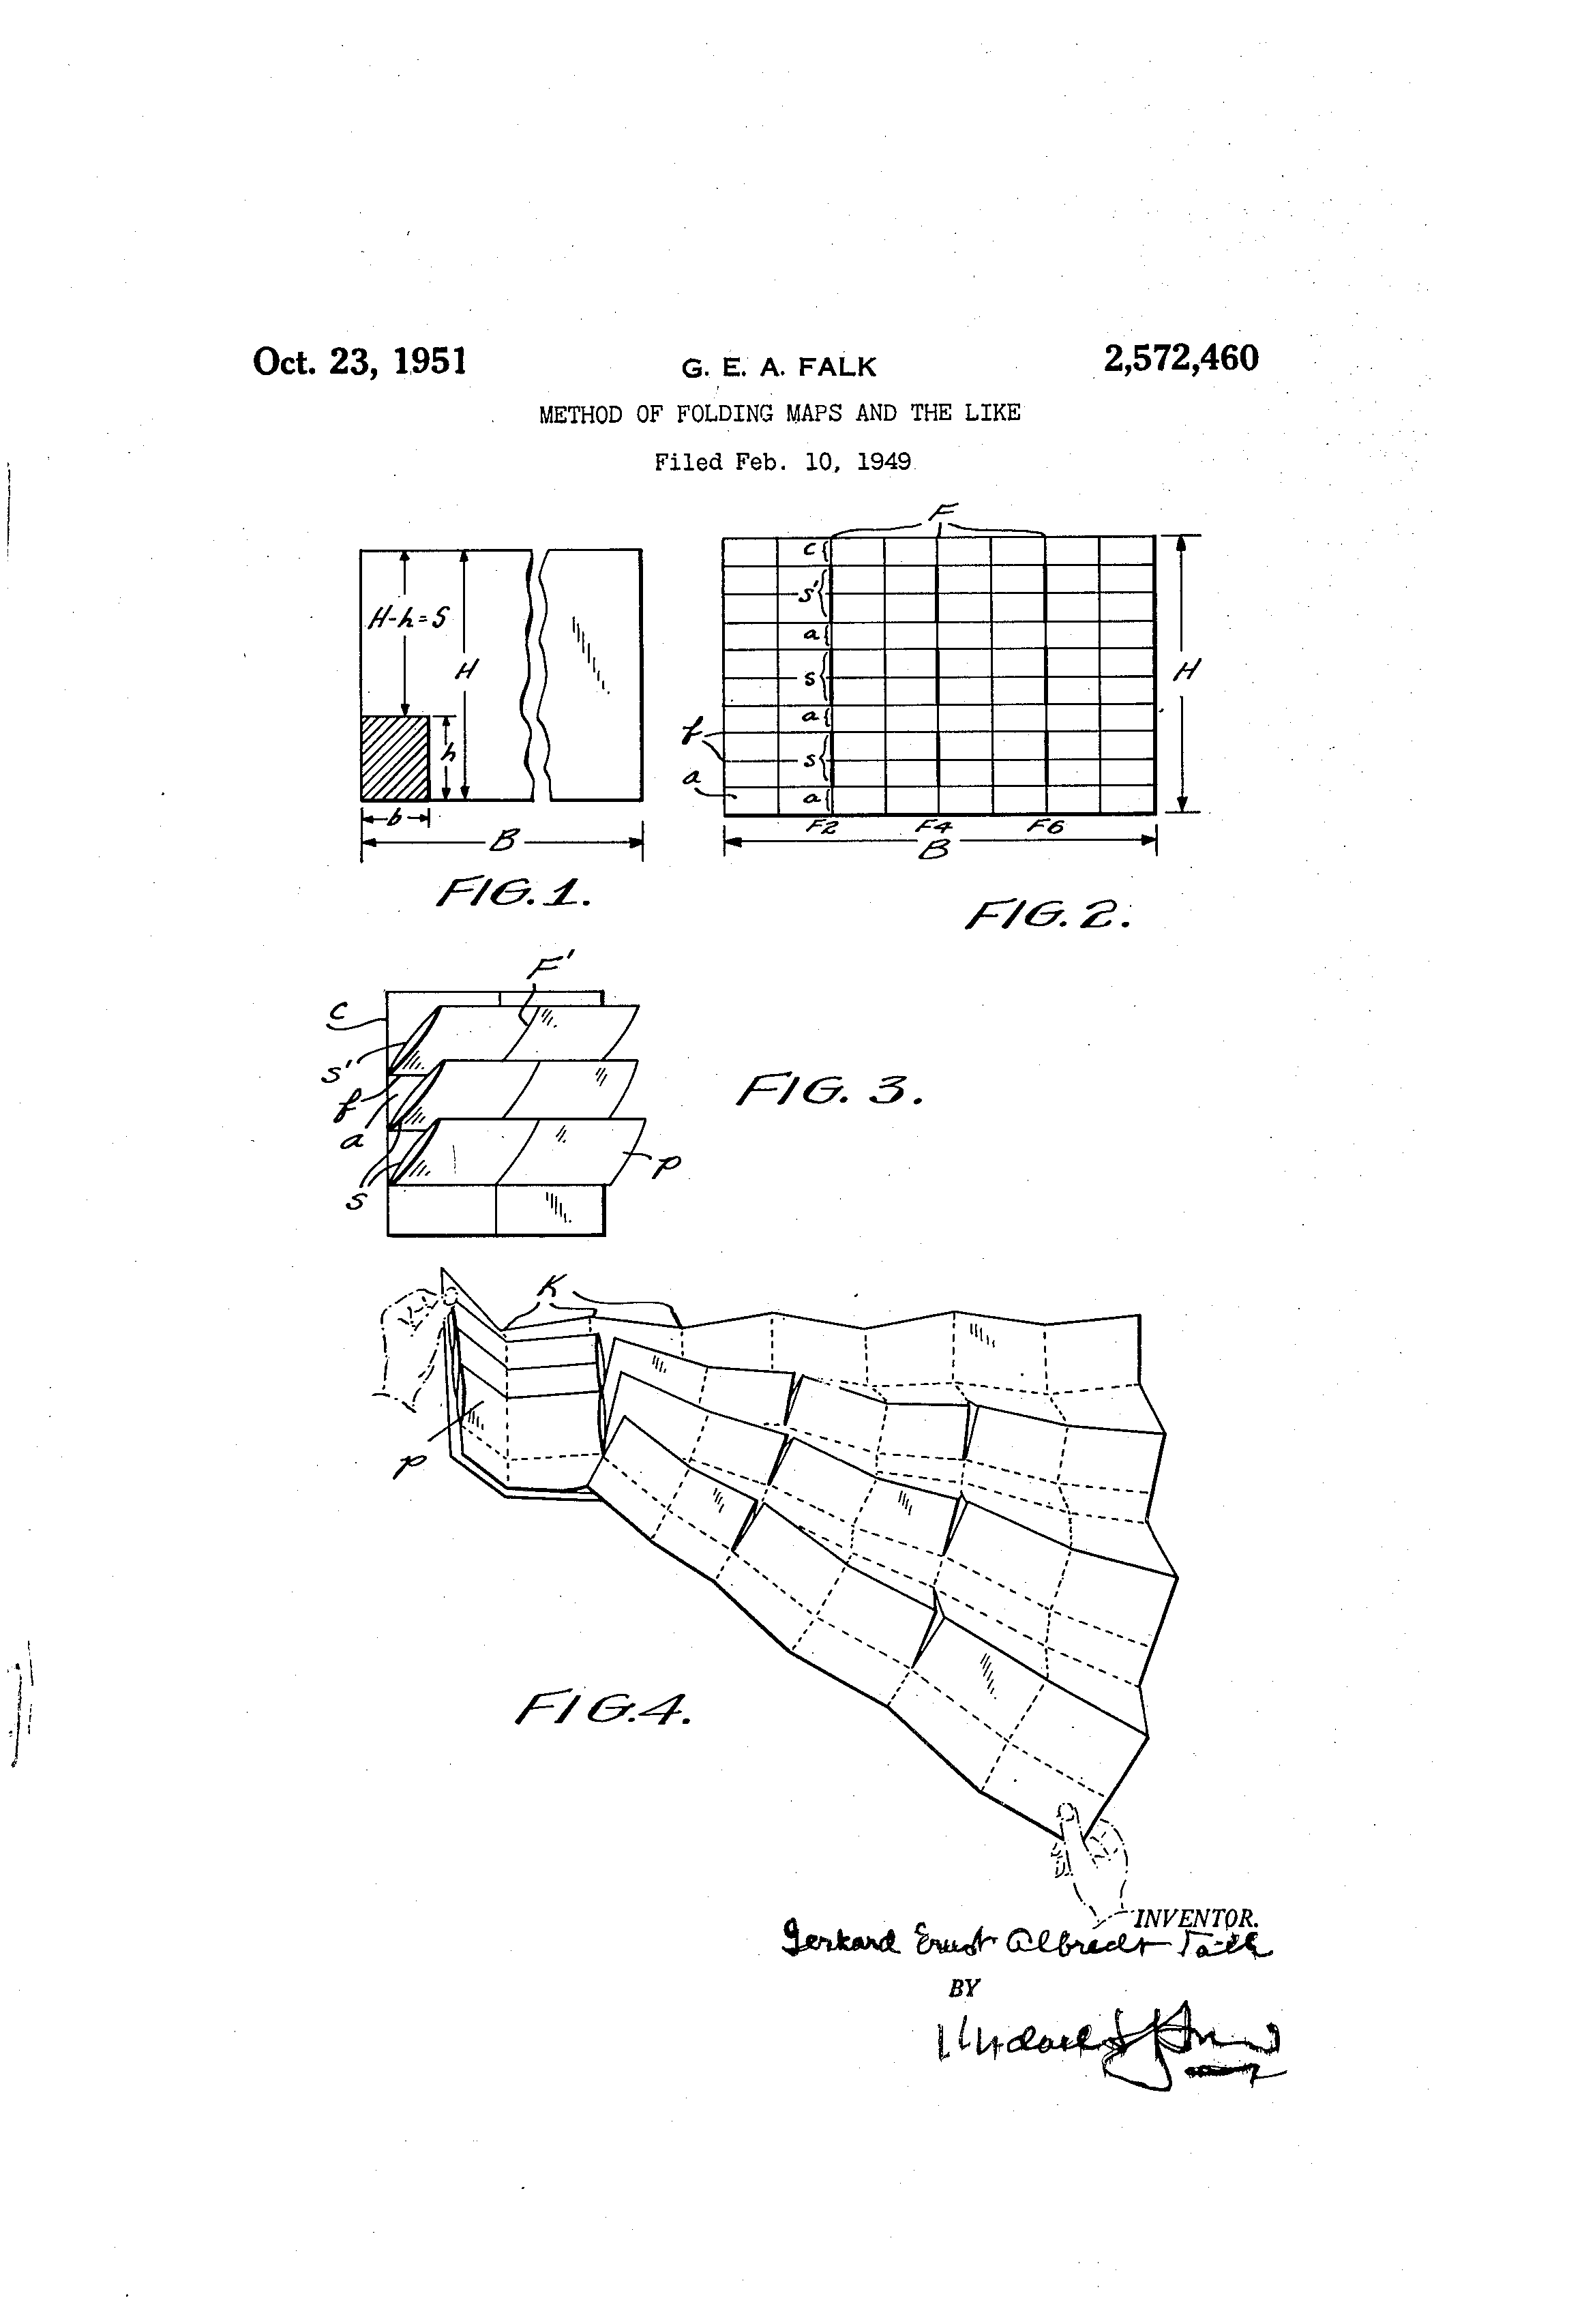
\includegraphics[width=\linewidth]{falk-patent.png}
  \caption{US Patent 2572460 \emph{``A United Method for Folding Maps and the Like''}, from 1951 by G. E. A. Falk, describes a technique for folding printed maps in such a way that they can be read without fully unfolding them.}
  \label{fig:falkmap}
\end{marginfigure}

In screen-based graphical user interfaces, these cases are usually handled by relying on clipping, \ie by employing a virtual space on which all of the information is laid out, and cutting off the content at the edges of the screen. Users can then interactively navigate the virtual space by moving their viewport, \eg by scrolling. This technique works, but it is sub-optimal, because it puts the burden of keeping track of the position in the virtual space on the user. Instead of being able to see the entire space they have to rely on their mental model of it \cite{bederson2011promise}.

Unlike with screens, there are no natural boundaries for Virtual Reality (\textsc{vr}) interfaces, because the virtual environment takes up the entire field of vision. Additionally, users can move around in this environment while using an application. This presents the opportunity to use the larger space, as well as the third dimension, in the design of user interfaces.

However, there are few examples of \textsc{vr} interfaces that make use of these possibilities. Most \textsc{vr} applications today are either games or novelty apps such as 3D drawing programs.
The interfaces with some complexity that do exist tend to mimic 2D interface patterns and employ clipping (see figure~\ref{fig:superhot}).

\begin{figure}
  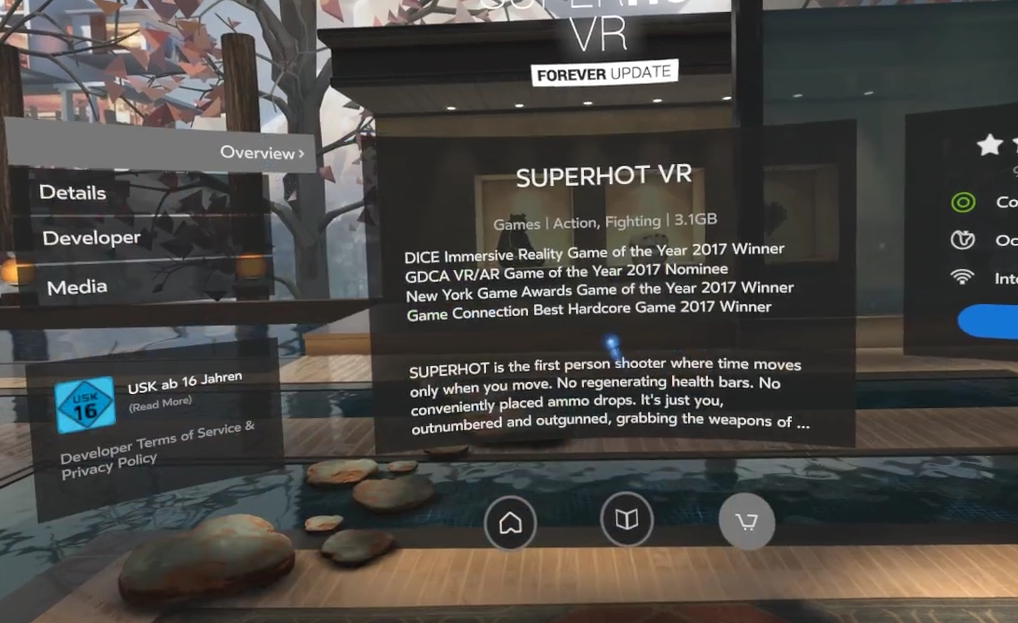
\includegraphics{superhot.png}
  \caption{Application detail page in the Oculus Home store. Clicking the sections on the left changes the content of the center column with a fade animation.}
  \label{fig:superhot}
\end{figure}

In this study we explored spatial interfaces which enable the presentation and navigation of large data sets using the unique possibilities that 3D space affords. While the limited real estate on screens necessitates clipping in most cases, this is not true for \textsc{vr}. The potentially unlimited 3D space \textsc{vr} interface elements exist in allows us to keep them around, even when they aren't being used or looked at.

% \begin{marginfigure}
%   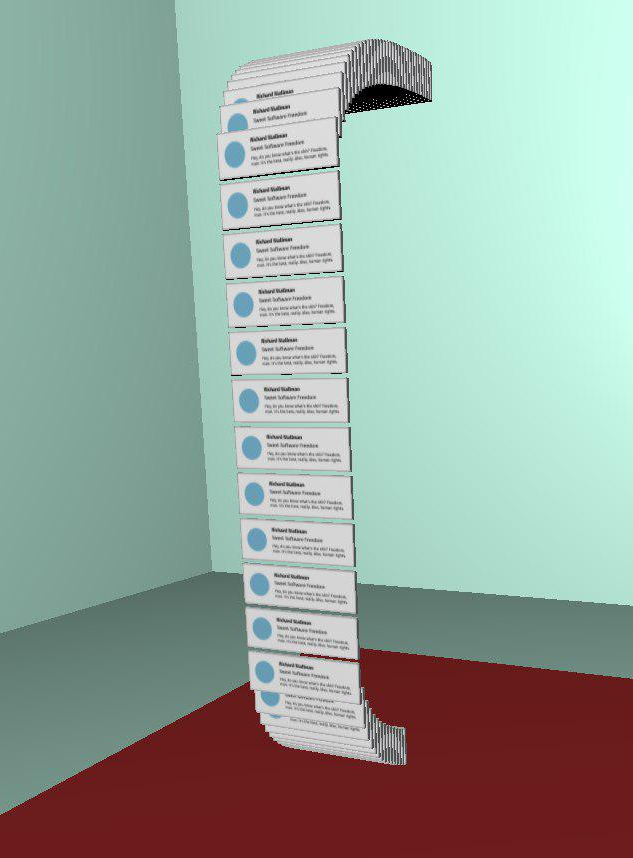
\includegraphics[width=\linewidth]{email.png}
%   \caption{Prototype of a list interface which stacks overflowing cards in the z-dimension.}
%   \label{fig:email}
% \end{marginfigure}

\subsection{Research Question}
The primary research question is whether spatial interfaces can improve the usability of \textsc{vr} applications compared to clipping. Additionally, we explored the advantages and disadvantages of different spatial approaches and interaction modalities in \textsc{vr}.

To answer our question we tested three different interfaces displaying the same information, two of which were spatial, while one employs clipping. We measured the performance of these different interfaces in a quantitiative experiment, and assessed the user experience using questionnaires.

\subsection{Contributions}
We evaluated general-purpose patterns for displaying and navigating large amounts of information in \textsc{vr}, which can be used by others building information-dense \textsc{vr} applications in the future.

%----------------------------------------------------------------------------------------
%	RELATED WORK
%----------------------------------------------------------------------------------------

\chapter{Related Work}
\label{ch:related-work}

This chapter aims to provide an overview of the history and state of the art in \textsc{vr} research, the most important challenges with designing \textsc{vr} interfaces, and the various interaction techniques that have been developed to overcome them. It also surveys the use of 3D space in the interfaces of current-generation consumer \textsc{vr} systems.

\section{Virtual Reality}
Both \emph{Augmented Reality} and \emph{Virtual Reality} use screens (or other display technologies) and positional tracking of the user's body in order to simulate virtual, spatial objects before the user's eyes. Azuma's \emph{Survey of Augmented Reality} (1997) describes Augmented Reality as ``3-D virtual objects are integrated into a 3-D real environment in real time'' \cite{azuma1997survey}. Virtual Reality, on the other hand, tends to be used to describe systems with few or no real-world objects, where users are fully immersed in an experience.


Milgram's reality-virtuality continuum spans from augmented reality (mostly real objects with some virtual ones), to virtual reality (mostly virtual elements) \cite{milgram1994taxonomy}. Between these two extremes there are many different types of \emph{mixed reality} with different degrees of virtuality.

\begin{figure}
  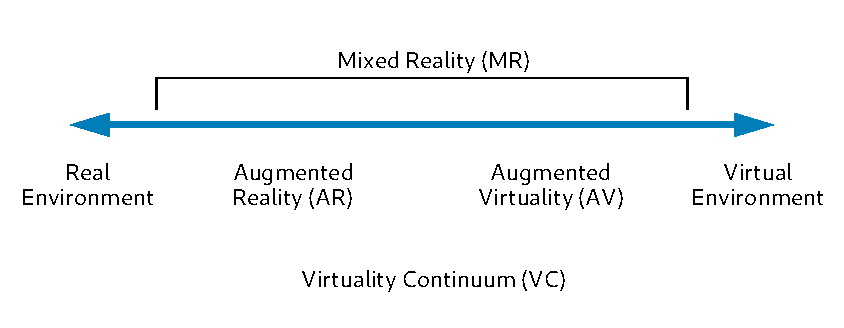
\includegraphics{milgram.pdf}
  \caption{A simplified representation of Milgram's reality-virtuality continuum.}
  \label{fig:milgram}
\end{figure}

\begin{figure}
  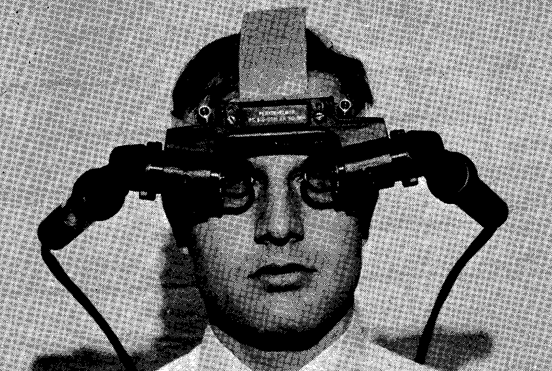
\includegraphics{sutherland-hmd.png}
  \caption{Ivan Sutherland's 1968 head-mounted display with miniature CRTs.}
  \label{fig:sutherland}
\end{figure}

\newpage

The earliest experiments with virtual and augmented reality date back as far as the 1960s \cite{sutherland1968head}, but only starting in the late 1980s head-mounted displays became practical and widely available \cite{billinghurst2015survey}. Though the technology was limited (both in terms of the display technology, and the graphics hardware used for rendering the virtual environments), many of the interaction techniques still used in current-generation \textsc{vr} were developed on these headsets.

Figure~\ref{fig:forte} shows the Forte VFX1, a head-mounted display released in 1995 \cite{fortevfx1}. It came with headphones and a handheld controller. The resolution was $263$ $\times$ $230$ pixels per eye, and the field of view $35.5$ degrees horizontally and $26.4$ degrees vertically.

\begin{figure}
  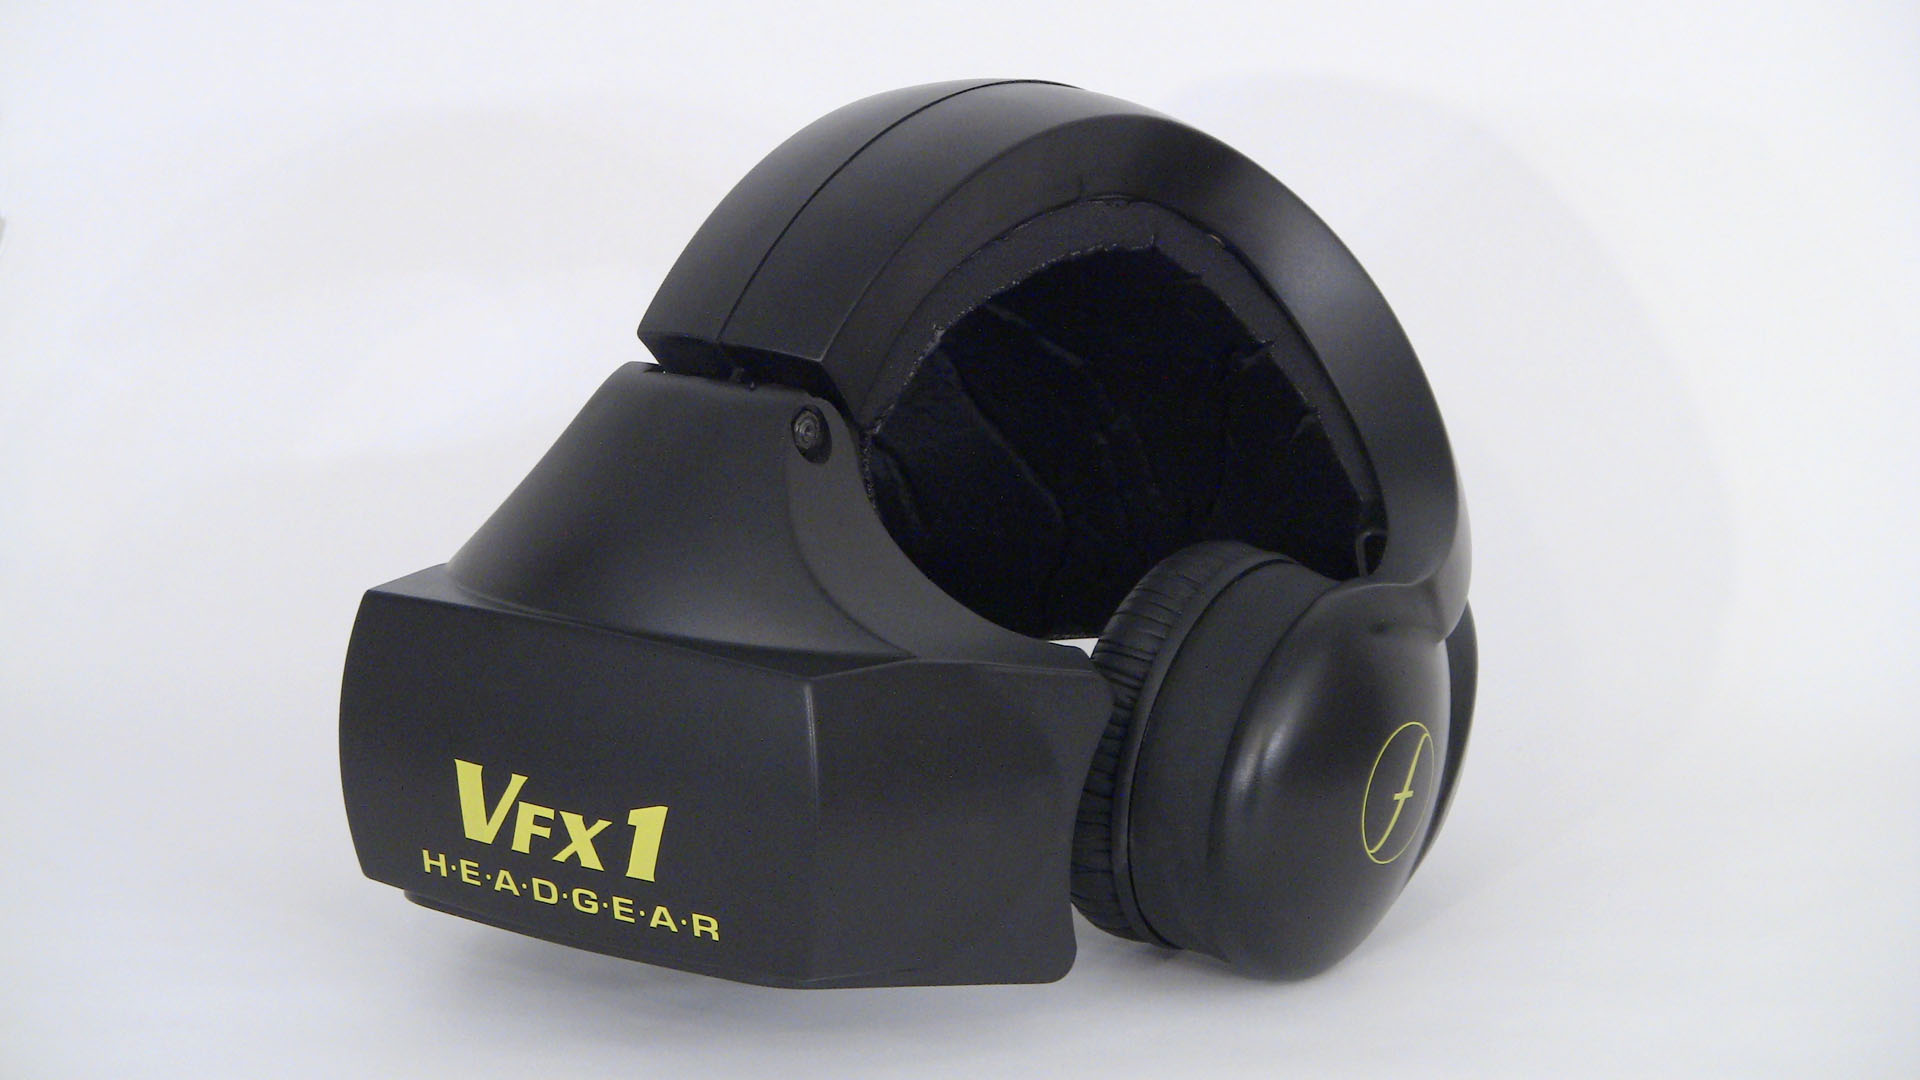
\includegraphics{forte-vfx1.jpg}
  \caption{The Forte VFX1, an early head-mounted display for virtual reality.}
  \label{fig:forte}
\end{figure}

The 1995 paper \emph{User interface constraints for immersive virtual environment applications} gives an overview of the interface design constraints and challenges when building \textsc{vr} interfaces \cite{bowman1995user}. It stresses the importance of affordances (and signifiers), mappings, feedback, and constraints to designing usable interfaces \cite{norman2013design}, especially in the context of immersive \textsc{vr} software. It mentions spatial boundaries that keep users from leaving the physical space designated for the \textsc{vr} experience, raycasting for object selection, and a number of other techniques that are still highly relevant in 2017.

\subsection{Input Devices}
When it comes to interacting with \textsc{vr} objects, the fundamental problem is that the ``natural'' way to interact with 3D objects in the real world using our hands does not work. \textsc{vr} headsets simulate the visual appearance of virtual objects, but there is no equally flexible technology for simulating haptics \cite{burdea1999keynote}, so \textsc{vr} objects cannot be touched or manipulated like real-world objects. Different \textsc{vr} input technologies have different sets of trade-offs, but are ultimately all limited in this respect.

The simplest interaction mechanic, mostly employed by mobile \textsc{vr} systems on phones, is gaze-based. To trigger an action, the user has to look at an object and either wait a certain amount of time, visualized by a ``fuse'' timer, or press a button on a remote to confirm the action. This mechanic is of course very limited and only useful for simple experiences like media consumption. Some \textsc{vr} experiences can be used with traditional game controllers, which provide more degrees of freedom and better haptic feedback, but are also very limiting because they can only be used for indirect manipulation. They also require remembering the button layout, because the controller is not visible from within \textsc{vr}.

\begin{figure}
  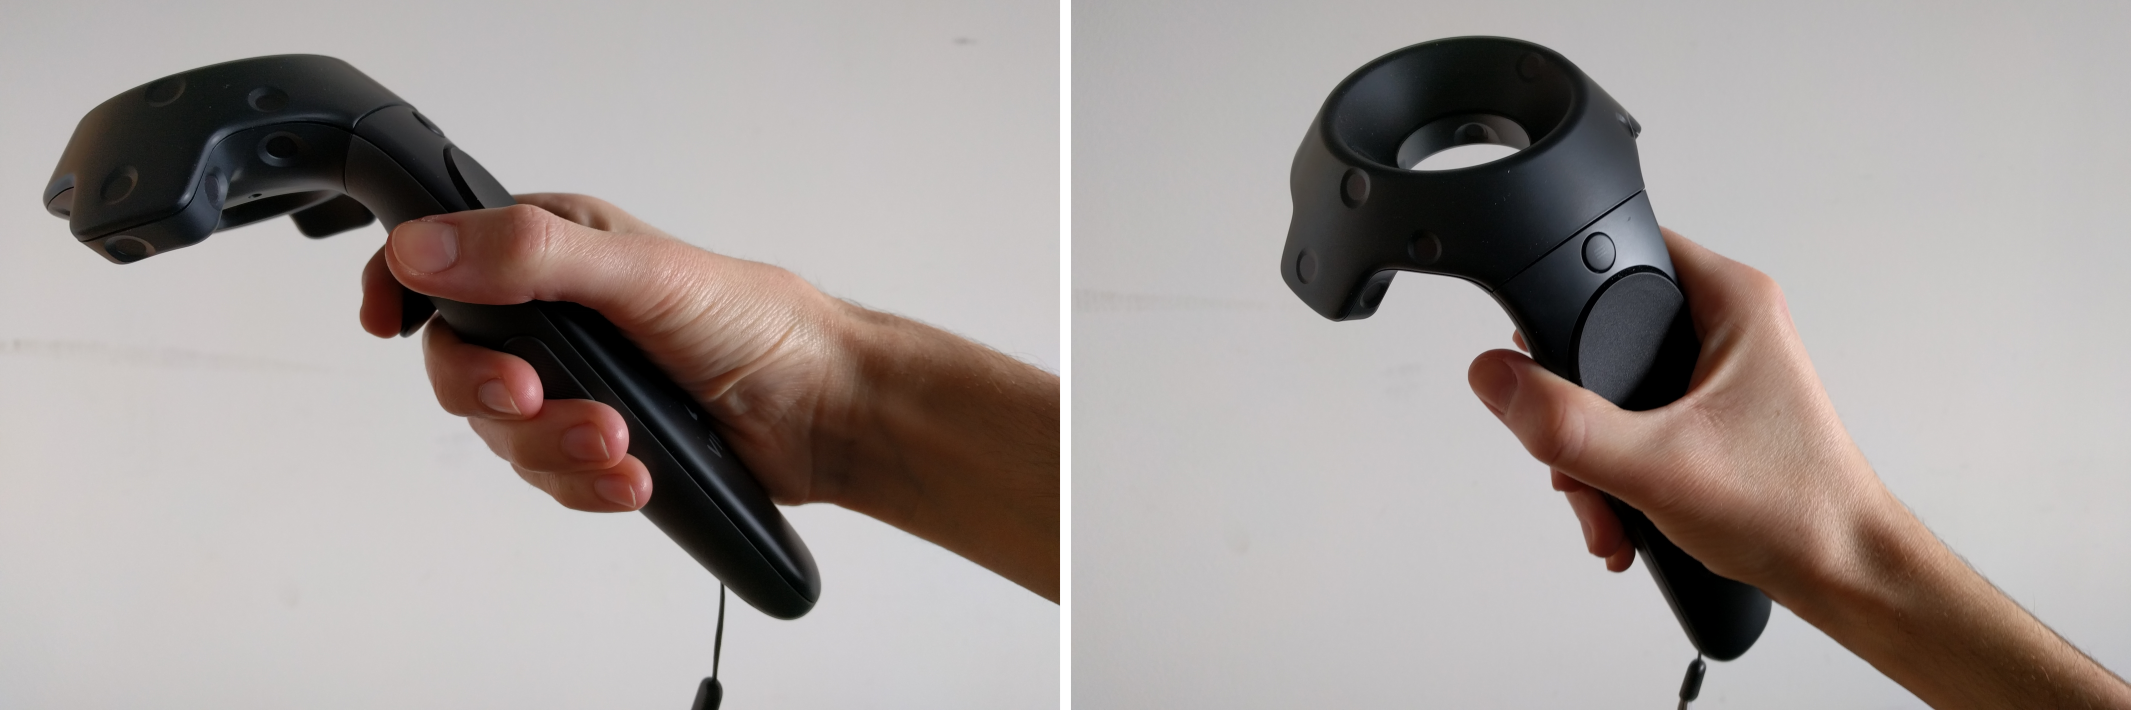
\includegraphics{vive-controller.png}
  \caption{How an HTC Vive controller is held, with the index finger on the trigger button (seen from the side and the top).}
  \label{fig:vive-controller}
\end{figure}

\textsc{vr} systems like the Oculus Rift or HTC Vive come with two controllers, one for each hand. They are tracked in 3D space, and are therefore visible in \textsc{vr}. Their shape and button layouts allow for some natural hand movements, like grabbing or pointing to be detected. Figure~\ref{fig:vive-controller} shows an HTC Vive controller. However, the current generation of controllers does not detect each finger separately, so this is limited to a few gestures. The spatial tracking of the controllers allows for some degree of direct manipulation of objects, e.g. moving the hand onto an object, grabbing it, and then throwing it across the room. There are limitations to this however, since there is no real haptic feedback, and objects offer no resistance to the user intersecting them with their bodies or controllers \cite{sanchez2005presence}.

Other systems, such as the Microsoft HoloLens, employ a gesture-based interaction model using hand tracking. This works by visually detecting hand positions and gestures using the cameras on the headset. It is also possible to add hand tracking to desktop \textsc{vr} systems such as the HTC Vive by adding a Leap Motion hand tracking system to it \cite[-1cm]{wozniak2016possible}. These systems have the advantage of not requiring additional hardware and allowing for more degrees of freedom. However, they lack any kind of haptic feedback and the gesture recognition can be unreliable, which is frustrating for users.

\begin{figure}
  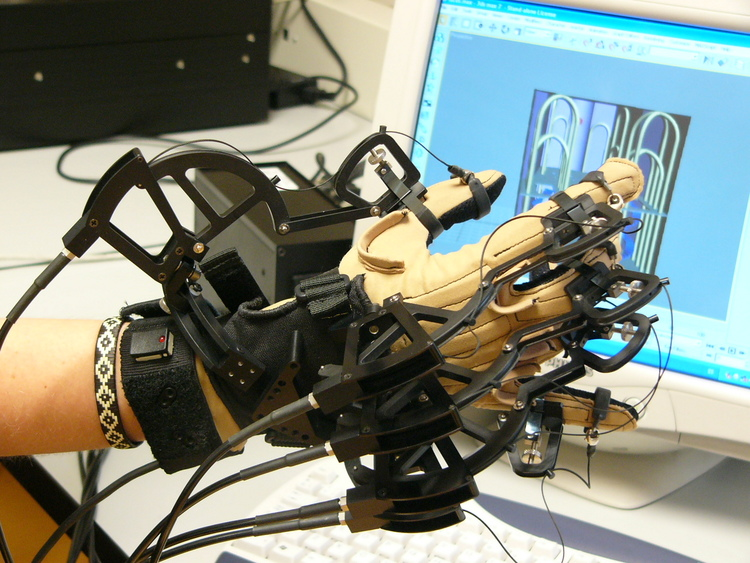
\includegraphics{cybergrasp.jpg}
  \caption{The CyberGrasp, consisting of the CyberGlove, a fabric glove containing sensors for the hand position, and an exoskeleton with cable-driven actuators to provide haptic feedback.}
  \label{fig:cybergrasp}
\end{figure}

% \begin{marginfigure}
%   \includegraphics[width=\linewidth]{pinchgloves.png}
%   \caption{Pinchgloves}
%   \label{fig:pinchgloves}
% \end{marginfigure}

Another possible type of input device is using gloves with sensors to track hand movements and gestures. This technology is not used by any current-generation \textsc{vr} system, but there have been several commercially available devices implementing this concept. Some of these devices did not actually track the motion of the fingers, but merely registered when two fingertips touched, and could therefore only recognize pinching gestures \cite{bowman2001pinchgloves}. More advanced solutions like the CyberGlove are able to precisely track hand movements movements, including the bend on each individual finger. This system can be extended to provide haptic feedback using mechanical actuators. However, this requires more than just a glove, but an exoskeleton around the user's hand \cite{bar2003haptic}. It is therefore not very practical for general-purpose systems, and mostly used for specialized industrial or military applications.

\subsection{Locomotion}
The simplest way to navigate \textsc{vr} experiences is tracking body movement and mapping it 1-1 to the virtual space. Current-generation room scale \textsc{vr} is capable of doing this reasonably well. Thanks to a 90 Hz display refresh rate (in both Oculus and Vive) there is no perceivable lag from head movement in most cases. However, this type of locomotion limits the size virtual spaces to the size of the physical space (usually around $3$ $\times$ $3$ meters for current-generation room scale \textsc{vr} systems). This means that the virtual spaces can not have arbitrary proportions, which is a problem for many kinds of \textsc{vr} experiences, such as open-world games, or architectural simulations. Thus, more flexible, but less intuitive types of locomotion are required in order to enable these kinds of experiences inside limited physical spaces.

One solution to this problem is ``flying'' around the virtual space by simply moving the camera without the user moving their body. The movement can be indirectly controlled e.g. by pressing buttons on a controller \cite{bowman1996evaluation}. This is a very flexible locomotion mechanic that scales to any kind of room, but is problematic because it can cause motion sickness. Since the user is not actually moving, it results in conflicting visual and vestibular stimuli, leading to disorientation and nausea for many people \cite{akiduki2003visual}.

Another common solution is teleportation. In most implementations of this mechanic, the user can set their new position by pointing at a location somewhere in the virtual space \cite{bozgeyikli2016point}. They are then instantly ``transported'' to the new location, usually with little or no animations. This can be disorienting, as the user has to re-scan the space after the transitions, but since there is no movement between the start and end positions, it does not cause motion sickness. The feedforward of explicitly setting the new position in space is likely another factor that mitigates this. Figure~\ref{fig:teleport} shows an example of what this looks like.

\begin{figure}
  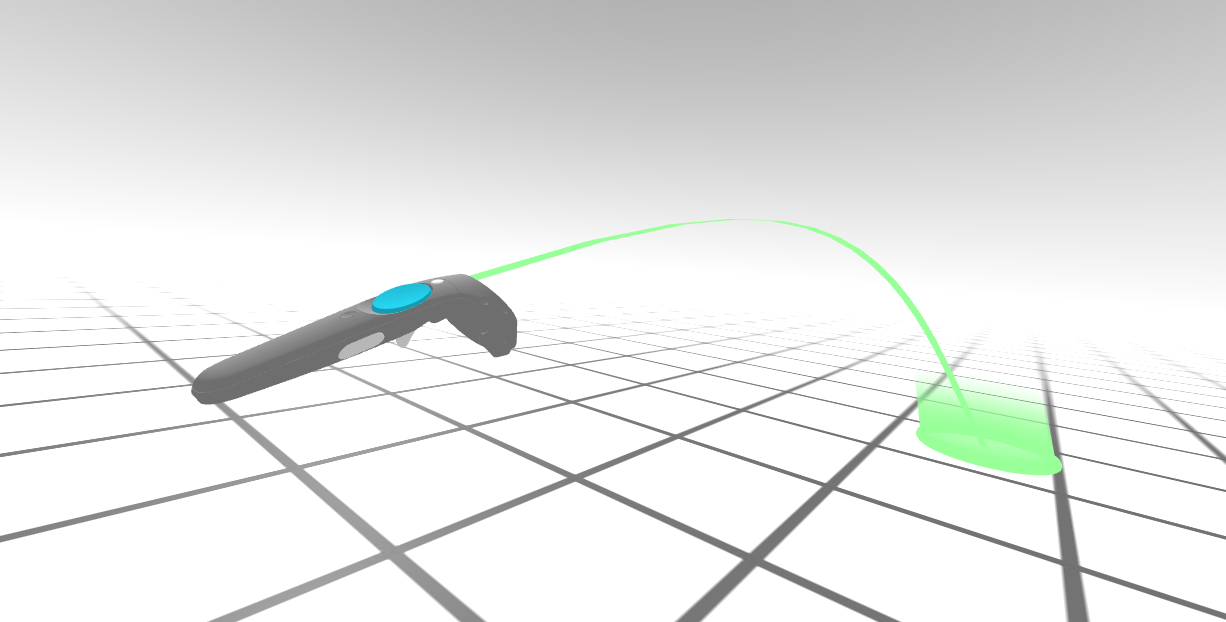
\includegraphics{teleport.png}
  \caption{The teleportation mechanic, as implemented by A-Frame's teleport component. The green circle on the floor previews where the user will be teleported.}
  \label{fig:teleport}
\end{figure}

\newpage

``Redirected Walking'' is a technique that imperceptibly rotates the virtual environment to accommodate a larger virtual space \cite{razzaque2001redirected}. This can be used to create the illusion of walking in a straight line, when in reality walking along an arc (see figure~\ref{fig:redirected}). However, since the rotation has to be slow in order for users not to notice it, this technique requires a large tracked space in order to accommodate arbitrary virtual environments.

\begin{figure}
  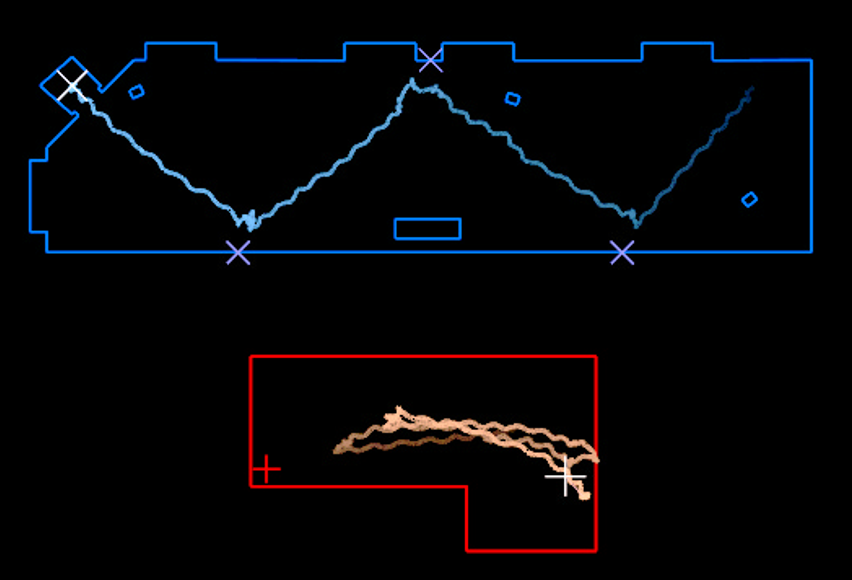
\includegraphics{redirected.png}
  \caption{Walking paths in the virtual environment (above in blue) and the real room (below in red) from the study by Razzaque et al. When the user stands still, the environment slowly turns their view of the virtual environment, turning the zig-zag path in \textsc{vr} into a a back-and-forth path in the real room.}
  \label{fig:redirected}
\end{figure}

Other approaches to this problem use specialized hardware to give users the illusion of physical travel. Omnidirectional treadmills allow users to walk in place without actually moving. This can be achieved using two perpendicular treadmills with a tracking system \cite[-3.3cm]{darken1997omni}, or a low-friction surface and special shoes \cite[-1cm]{warren2017omni}.

\subsection{Selection \& Manipulation}
Basic direct manipulation of objects is possible with current-generation \textsc{vr} controllers, but sometimes indirect manipulation is necessary or preferable (e.g. because it is faster or more precise for a specific task). Bowman \& Hodges describe a design metaphor for indirect manipulation interfaces in \textsc{vr}  based on traditional desktop interface concepts such as widgets, menus, buttons, icons, and pointing \cite{bowman1994wimp}.

Most \textsc{vr} interfaces today employ patterns like these (see figure~\ref{fig:earth-menu}), which are translations of 2D interface elements to the 3D environment. Instead of a mouse pointer, raycasting cursors starting from a hand-tracked controller are often employed to select items. Clicks are emulated by button presses while an object is selected via raycasting. In this way, most traditional desktop interface elements, such as buttons, sliders, and switches can be used in 3D just as they would be in 2D.

\begin{figure}
  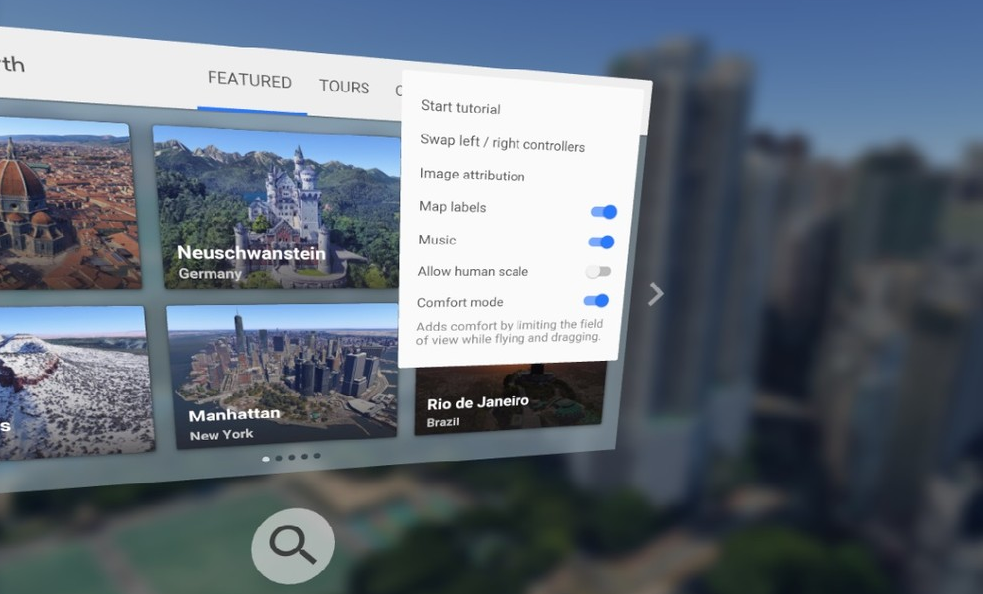
\includegraphics{earth-menu.png}
  \caption{A menu in Google Earth \textsc{vr}. The interface elements (tabs, menus, switches) are the exact same ones Google uses in their desktop and mobile products.}
  \label{fig:earth-menu}
\end{figure}

A different approach suggested by literature is using virtual ``tools'' to perform actions. Bowman defines these as ``specialized objects, in some ways not part of the environment itself, but rather the representations of methods the user may employ to perform actions on or in the environment'' \cite{bowman1995user}. Examples of virtual tools include guns or swords in games, paintbrushes in drawing applications, or minimaps of the environment to quickly teleport somewhere else. Wloka et al. present the Star Trek tricorder as a model for a multi-functional virtual tool, serving both as an input mechanism and a display \cite{wloka1995virtual}.

\newpage

Non-linear mapping of hand movement (also known as the ``go-go'' technique) has been proposed to make direct manipulation of far away objects less cumbersome \cite{poupyrev1996go}. Within a certain distance from the user, the virtual representation of the user's hands is directly mapped to their real hands. After this threshold, the virtual hands are mapped in a non-linear fashion, allowing users to reach further than they otherwise could.

A 1997 study evaluated six different techniques for manipulating remote objects, including go-go and raycasting \cite{bowman1997evaluation}. Based on the findings from this, study the \textsc{homer} technique (Hand-centered Object Manipulation Extending Ray-casting) was developed, a hybrid between raycasting and direct manipulation. In this technique the user first selects their target object using ray-casting. Their virtual hand is then moved to the object, allowing them to direcly manipulate it from a distance.

\begin{figure}
  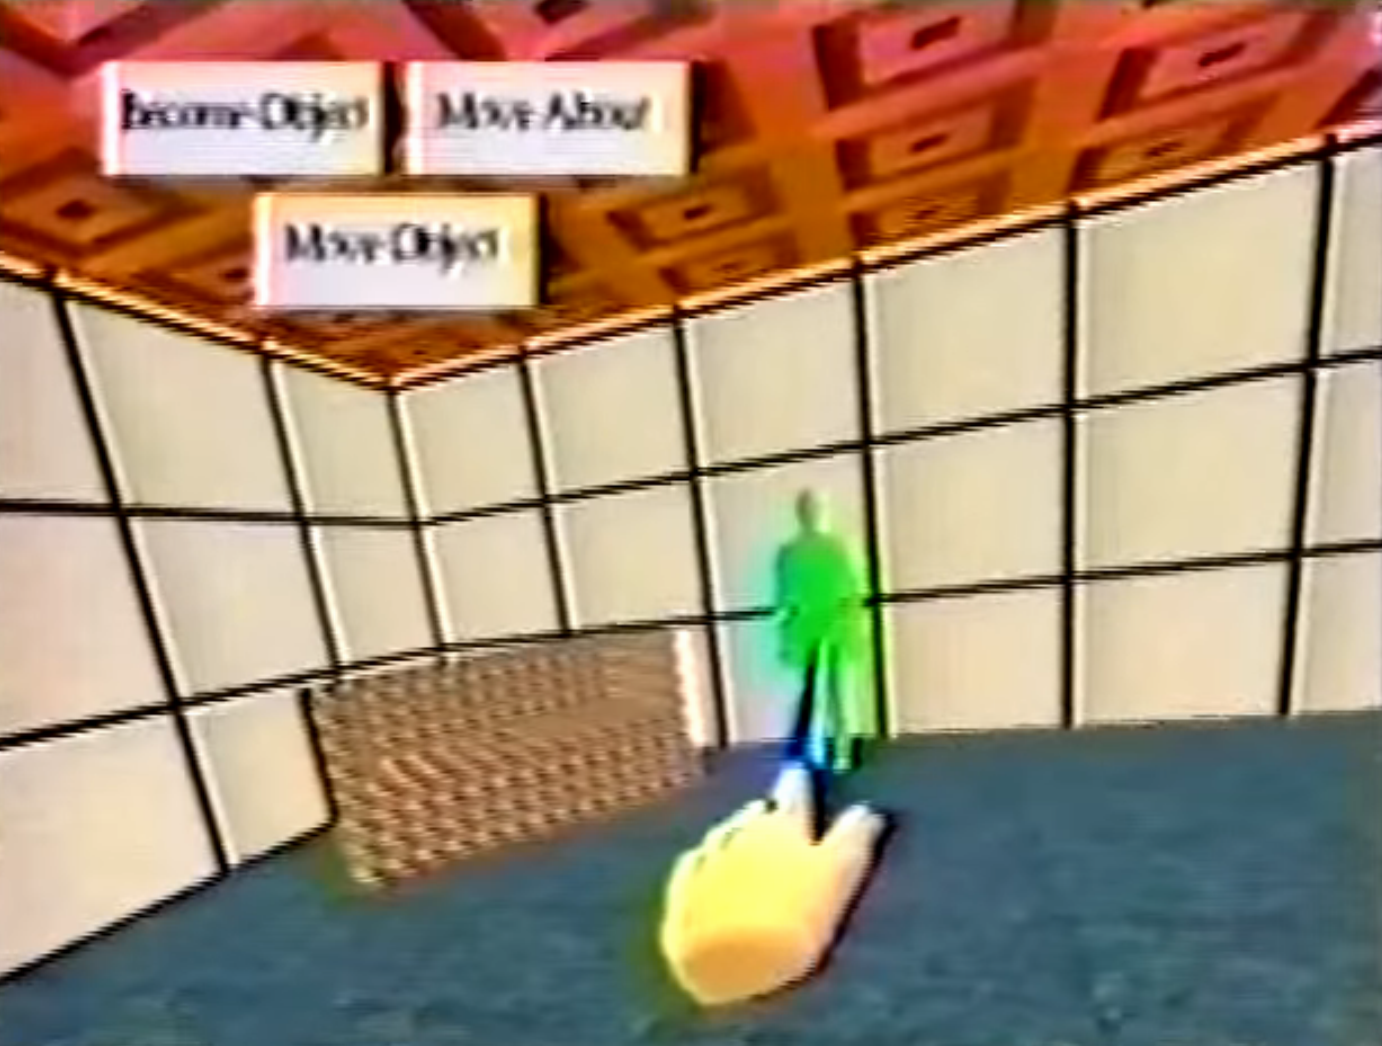
\includegraphics{homer.png}
  \caption{The selection stage of Bowman's \textsc{homer} technique. The element about to be selected is highlighted in green. After selection, the object can be moved in the environment using direct manipulation.}
  \label{fig:homer}
\end{figure}

Traditional raycasting does not work the selection of objects that are partially or fully occluded. The Flexible Pointer technique tracks both hands to interactively construct a bezier-like curve, which can be used to reach around the objects obscuring the target \cite{feiner2003flexible}.

\section{State of the Art \textsc{vr} Interfaces}
The current generation of \textsc{vr} Interfaces does not make much use of 3D space. Most interfaces are flat 2D panels, not very different from traditional 2D interfaces in both form and behavior. They rely heavily on flat, clipped, scrollable areas, or simply pagination with fade transitions (see figure~\ref{fig:steamstore}). The third dimension is often used for purely aesthetic purposes, e.g. as a three-dimensional wallpaper behind or around the interactive interface elements.

\begin{figure}
  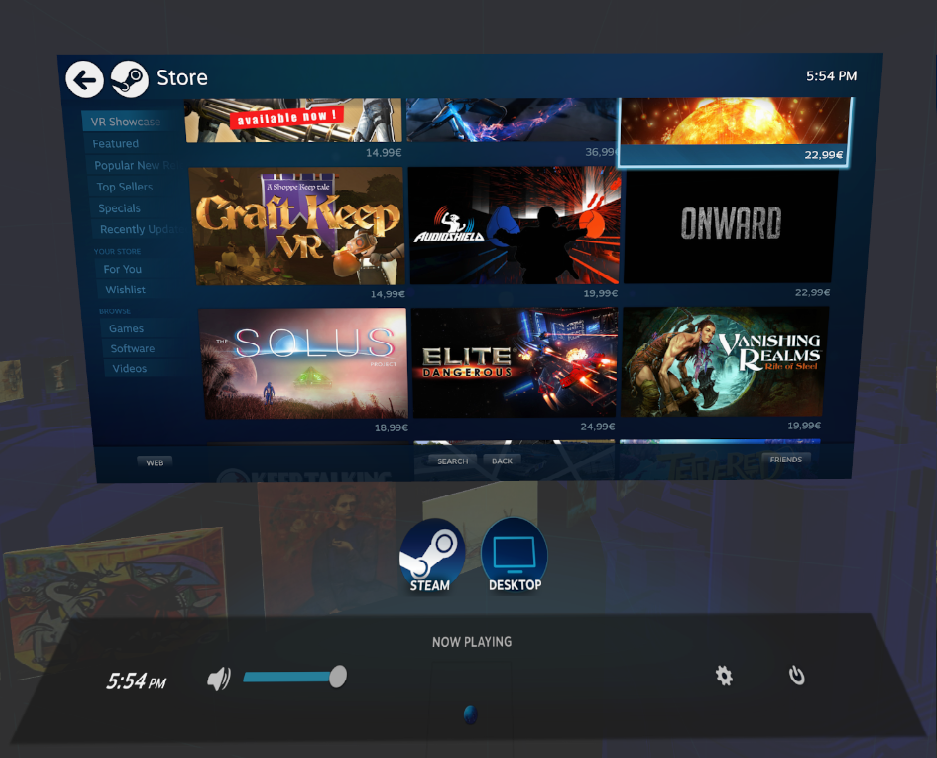
\includegraphics{steamstore.png}
  \caption{The SteamVR store interface is a single flat surface that behaves like a regular desktop app. On the bottom there is a taskbar to switch between open apps, and a system bar with time, volume and settings.}
  \label{fig:steamstore}
\end{figure}

When interfaces do use 3D, it is often in a highly skeuomorphic context, mimicking real-world interactions such as picking up items and throwing them.
This is at least in part due to the fact that the low resolution on the current generation of headsets makes interfaces high information densities impossible.

We found this to be true for both leading \textsc{vr} operating systems (Oculus Home and SteamVR), as well as most applications on these platforms. Oculus Home's interface makes some use of the 3D space by employing interface elements floating freely in space, while SteamVR's interface relies mostly on monolithic flat panels that behave exactly like a traditional screen. However, SteamVR has more consistent, spatial animations, while Oculus Home relies heavily on jarring cuts and fades.

\subsection{Controller-Mapped Interfaces}
One notable exception to the generally flat and traditional interfaces are the controls persistently mapped to the controllers in some applications. Google Earth and TiltBrush are prominent examples of this pattern, which is a variation of Bowman's concept of virtual tools \cite[-1cm]{bowman1995user}.

In TiltBrush, the left hand has a persistent menu with three pages of settings, which are arrayed around the controller, facing outwards (see figure~\ref{fig:tiltbrush}). They can be turned along the center axis with the left hand controller's touchpad, and the right hand controller is used to operate the menus.
The contents of the two menu panels not facing the user is not visible, likely so as not to be visually distracting. As the panels turn, only the one facing the user shows
The menus themselves are not as interesting as their containers, employing standard 2D interface patterns such as pagination and clipping.

In Google Earth, a miniature globe is fixed on top of the left hand controller (see figure~\ref{fig:globe}). The right hand controller can be used to point at a position on the globe to teleport there. This kind of navigation with two hands feels very intuitive, because it only relies on direct hand movement in space, not abstract button mappings or external controls. This mechanic implements Stoakley's World In Miniature (\textsc{wim}) concept \cite[-2cm]{stoakley1995virtual}.

\begin{figure}
  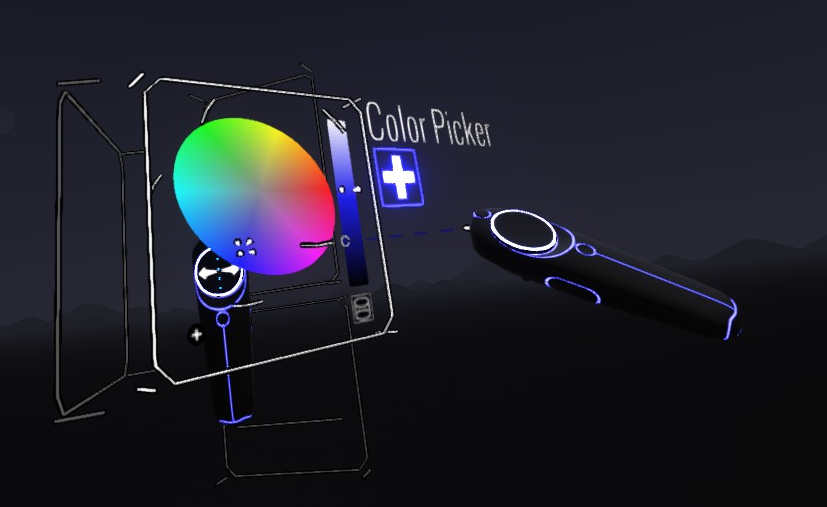
\includegraphics{tiltbrushmenu.png}
  \caption{The color picker page on the TiltBrush menu. Only the page facing the user contains actual content, while the other two are only visible as wireframe outlines.}
  \label{fig:tiltbrush}
\end{figure}

\begin{marginfigure}
  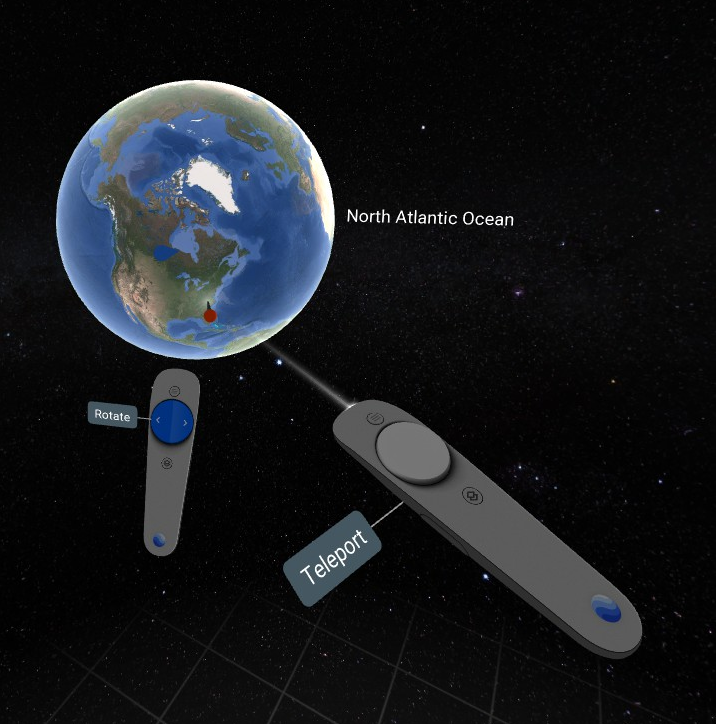
\includegraphics[width=\linewidth]{globe.png}
  \caption{The miniature globe is fixed to the top of the left hand controller and increases in size when pointed at by the right hand controller. A little red pin shows the location hovered by the cursor. Pressing the trigger button teleports to that location.}
  \label{fig:globe}
\end{marginfigure}

These examples show the potential of spatial interfaces in \textsc{vr}. They make use of the fact that users can see and move their hands, and move around the space. They make use of unique possibilities that 3D space offers in a functional way, to makes interfaces easier to navigate.

%----------------------------------------------------------------------------------------
%	BACKGROUND
%----------------------------------------------------------------------------------------

\chapter{Background}
\label{ch:background}

\section{Technology}
The \textsc{vr} ecosystem is currently (mid 2017) still in its infancy. We experimented with the Oculus Rift \textsc{cv1} and the \textsc{HTC} Vive (both released in early 2016) and tested the headset and controller hardware, software ecosystem, and developer tools.

The installation and setup are very cumbersome for both headsets, especially on the software side, where we encountered many glitches, bugs, and usability problems.

The biggest issue with both headsets is the very low resolution of only $1080$ $\times$ $1200$ pixels per eye. In addition, in the periphery of the display the picture is quite blurry. This means that refocusing the eyes to the sides to see content there is not possible, which is irritating. Text needs to be either very big, or very close in order to be legible, which makes any kind of information-dense application impractical \cite{elliott2015virtual}. Bowman's vision of Information-Rich Virtual Environments \cite{bowman2003information} is therefore still not feasible with current hardware.

Both the Rift and the Vive have room scale tracking that works reasonably well, but we found the Vive tracking to be more reliable. This is likely due to its trackers being mounted higher up and on opposite sides of the room. Walking around in the roughly 2x2m space feels natural, but the limitations of being able to move only within such a small space quickly become clear in scenarios like games with open-world environments, where it means that teleporting has to be the primary means of movement.

\section{Development}
We developed our prototypes in WebVR using Mozilla's A-Frame\footnote{A-Frame: A Javascript framework for building \textsc{vr} experiences on the web (https://a-frame.io)} Framework. A-Frame is a Javascript library which enables building \textsc{vr} experiences using declarative components directly in \textsc{html}. Its entity-component structure makes it easy to prototype experiences by combining existing components, and defining new ones in Javascript. A-Frame runs completely standalone in the browser (though it does require Steam or Oculus being set up on the computer in order to work with the Vive or Oculus headsets), and can be used with other Javascript libraries and standard web tooling. Though there are some performance and stability issues in some cases, the quality of the experiences is more or less on par with native \textsc{vr} for simple applications.

\section{Prototypes}
In an initial exploration phase, we designed a number of different spatial interfaces and built prototypes to test their viability. The goal was to find novel ways of using three dimensions to make \textsc{vr} interfaces that don't require clipping to display large amounts of information.

\subsection{Stacked List Prototype}
This prototype is a scrollable 1-dimensional list of cards which uses z-depth to stack cards at both ends of a list (see figure~\ref{fig:emailscroll}). The content of these stacked cards is not visible, but their presence shows how many items there are above and below the currently visible cards, thereby intuitively communicating the position in the list to the user, without relying on external indicators such as scrollbars.

\begin{figure}
  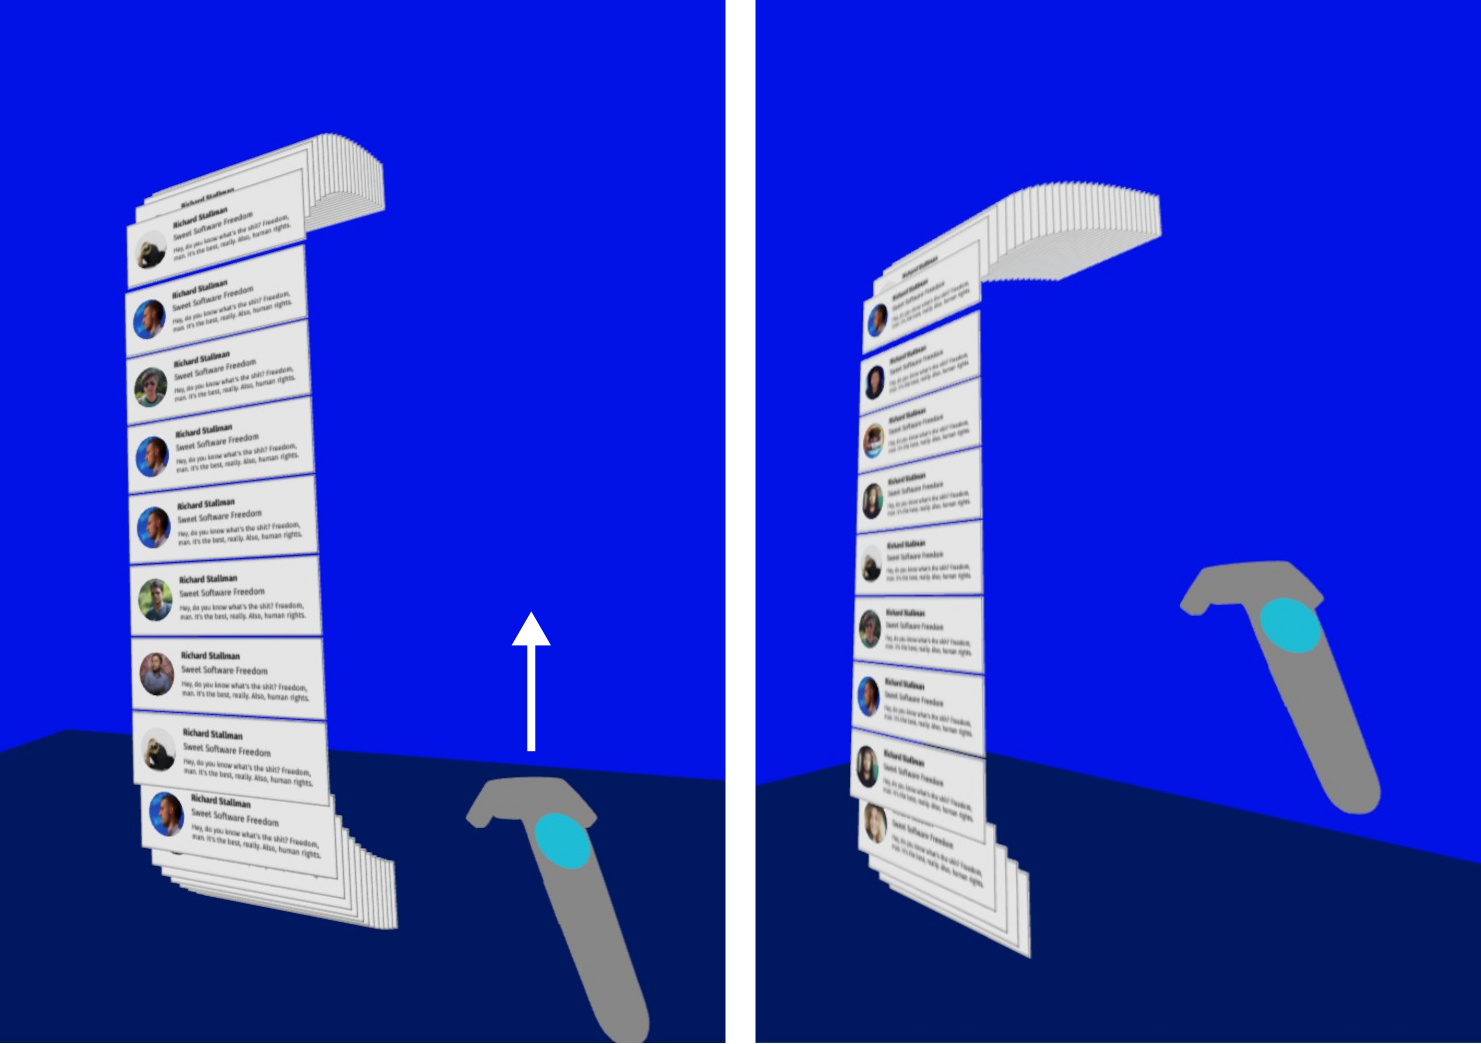
\includegraphics{emailscroll.png}
  \caption{Illustration of the scrolling behavior: Lifting up the controller while pressing the trigger button moves the cards up in the list.}
  \label{fig:emailscroll}
\end{figure}

The list can be scrolled by keeping the trigger button on the controller pressed while moving it vertically. The scrolling direction mimics the ``natural'' scrolling behavior on touchscreens and touchpads, whereby moving the controller up will move the elements upwards, thus scrolling down in the list.

The advantage of this approach is that it can accommodate many elements in a relatively small space. On the other hand, the usefulness of the stacked cards highly depends on the content. If the content is not very visually distinctive, individual cards are not recognizable while stacked.

This prototype was the inspiration for the \emph{Stacked} interface type in our study.

\subsection{Elevator Prototype}
In an attempt to use the available physical space as efficiently as possible, this prototype arrays information on a vertical 3D tube around the user (see figures~\ref{fig:picassoinside} and \ref{fig:picassooutside}). The information on the walls can be explored by walking around inside the tube, as well as changing the vertical position of the tube by interactively ``scrolling'' up and down, behaving as kind of elevator through the virtual space.

\begin{marginfigure}
  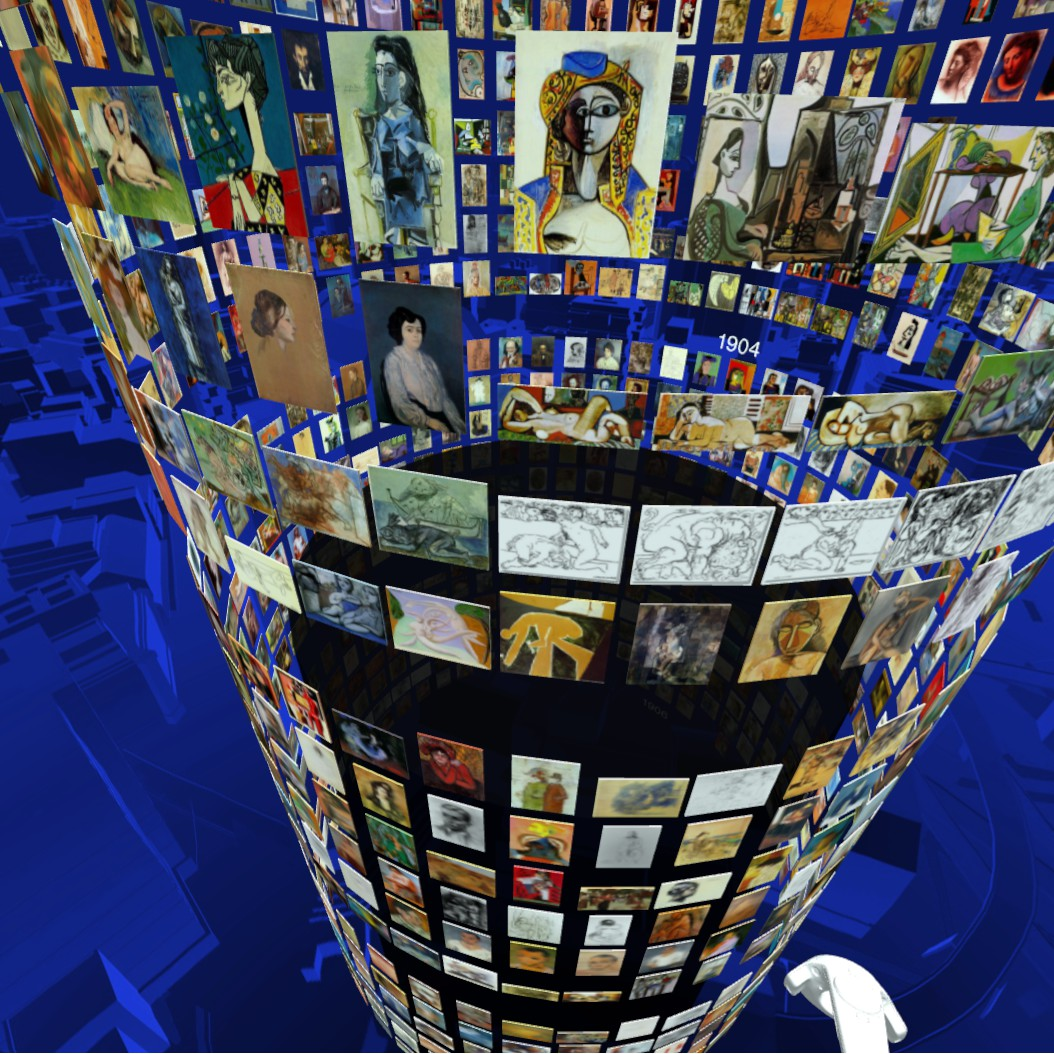
\includegraphics[width=\linewidth]{picassooutside.jpg}
  \caption{The ``elevator'' prototype, seen from the outside}
  \label{fig:picassooutside}
\end{marginfigure}

This prototype can accommodate very large amounts of information, and navigation is efficient and intuitive. However, being totally enveloped by the content can make orientation difficult due to the lack of stable landmarks. It also means that there is no possibility of getting a good overview by stepping back a bit. These problems could be addressed by only using having content along half of the tube. This could be combined with an overview mode, where the elevator moves back horizontally so users can see the tube from afar.

We found that most of the value in this kind of interface comes from being able to explore by simply looking around the space, rather than interacting. This is what inspired the \emph{Spatial} interface type in our study.

\begin{figure}
  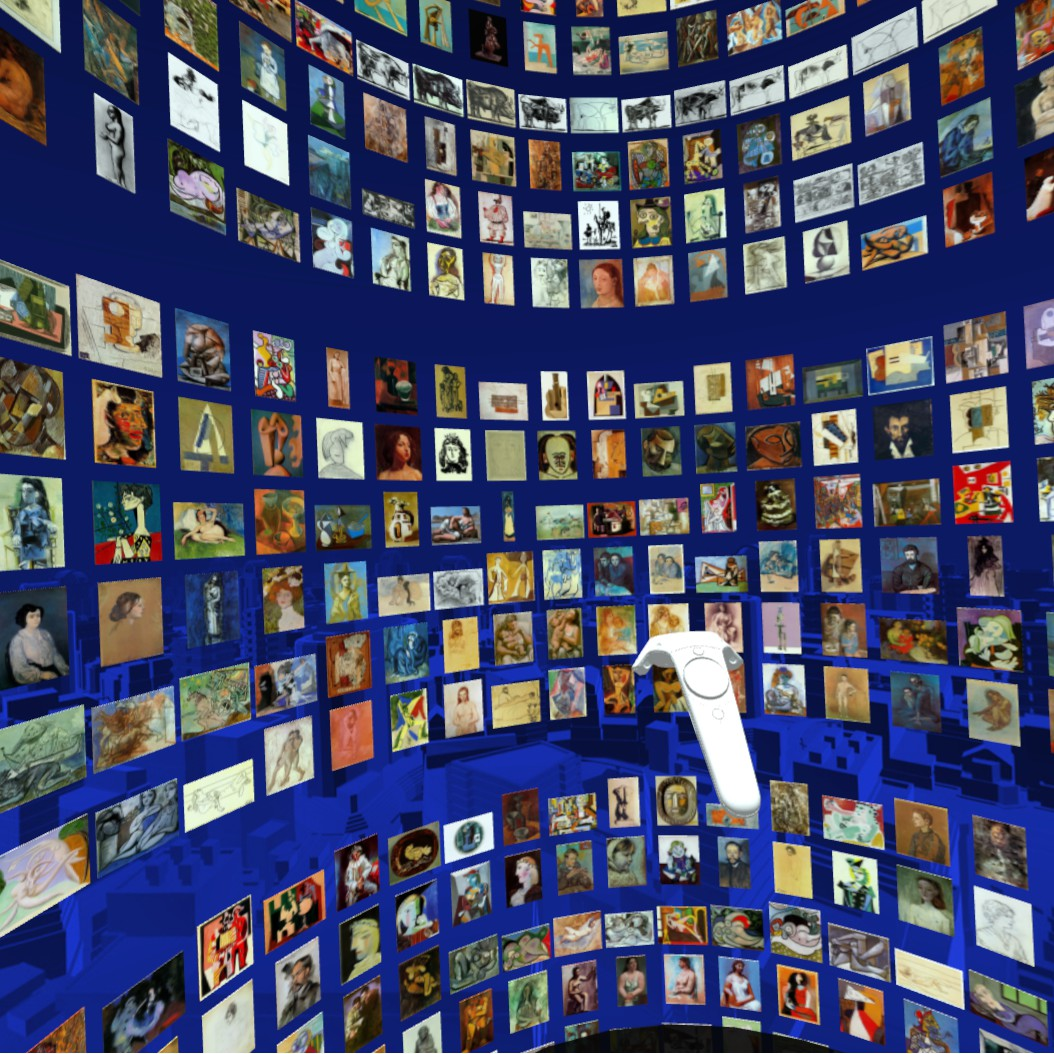
\includegraphics[width=\linewidth]{picassoinside.jpg}
  \caption{The ``elevator'' prototype showing paintings on the walls of the cylinder. The vertical position can be moved by pressing the trigger button and moving the controller vertically.}
  \label{fig:picassoinside}
\end{figure}

%----------------------------------------------------------------------------------------
%	EXPERIMENTS
%----------------------------------------------------------------------------------------

\chapter{Study}
\label{ch:study}

To evaluate the differences between spatial and clipping-based interfaces we conducted an empirical user study. We asked participants to perform the same task, finding icons in a list, using three different interfaces: A two-dimensional grid (\emph{Spatial}), a scollable list that stacks overflowing elements in the z-dimension (\emph{Stacked}), and a clipped, scrollable list (\emph{Clipped}), illustrated in figure~\ref{fig:experiment-types}.

\begin{figure}
  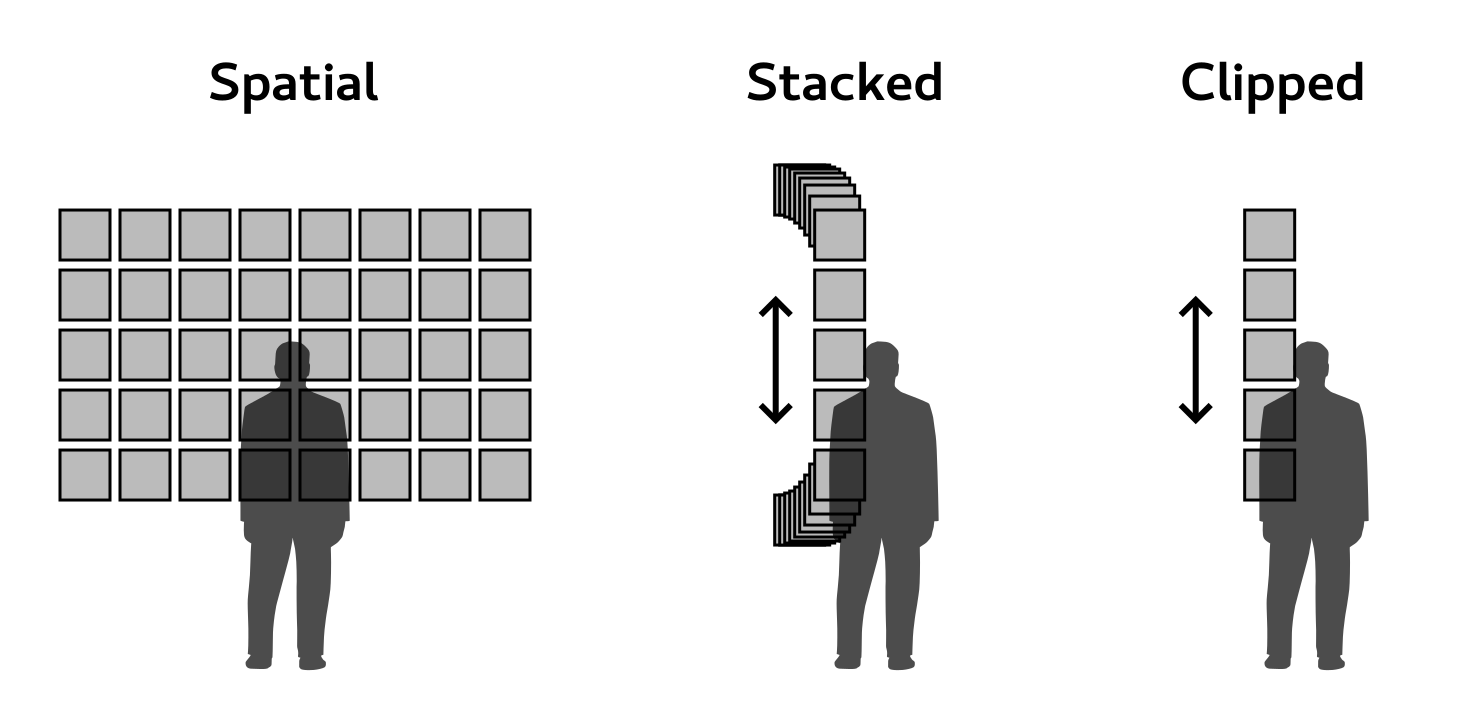
\includegraphics{types.png}
  \caption{The three different experiment types. Each of these was used in 6 different configurations, with different numbers of items, \emph{Colored} or \emph{Monochrome}.}
  \label{fig:experiment-types}
\end{figure}

\section{Participants}
We recruited 20 paid participants (8 female, 12 male), aged between 19 and 49 years (MDN = 24 years). Most of them were display workers, with an average of 5.9 hours per day working with computers (SD = 2.3 h). Most participants had some experience with Virtual Reality, but none of them had used it extensively.

\section{Apparatus}
The study was conducted in a university lab room using an HTC Vive connected to a Windows 10 PC. Participants were instructed to stand in the middle of an area measuring about $3m \times 3m$ at the center of the room. They were given the Vive headset and one tracked hand controller. The room scale \textsc{vr} setup allowed them to freely move within this area and have their body and hand movement reflected faithfully inside \textsc{vr} (see figure~\ref{fig:participant-view}).

\begin{figure}
  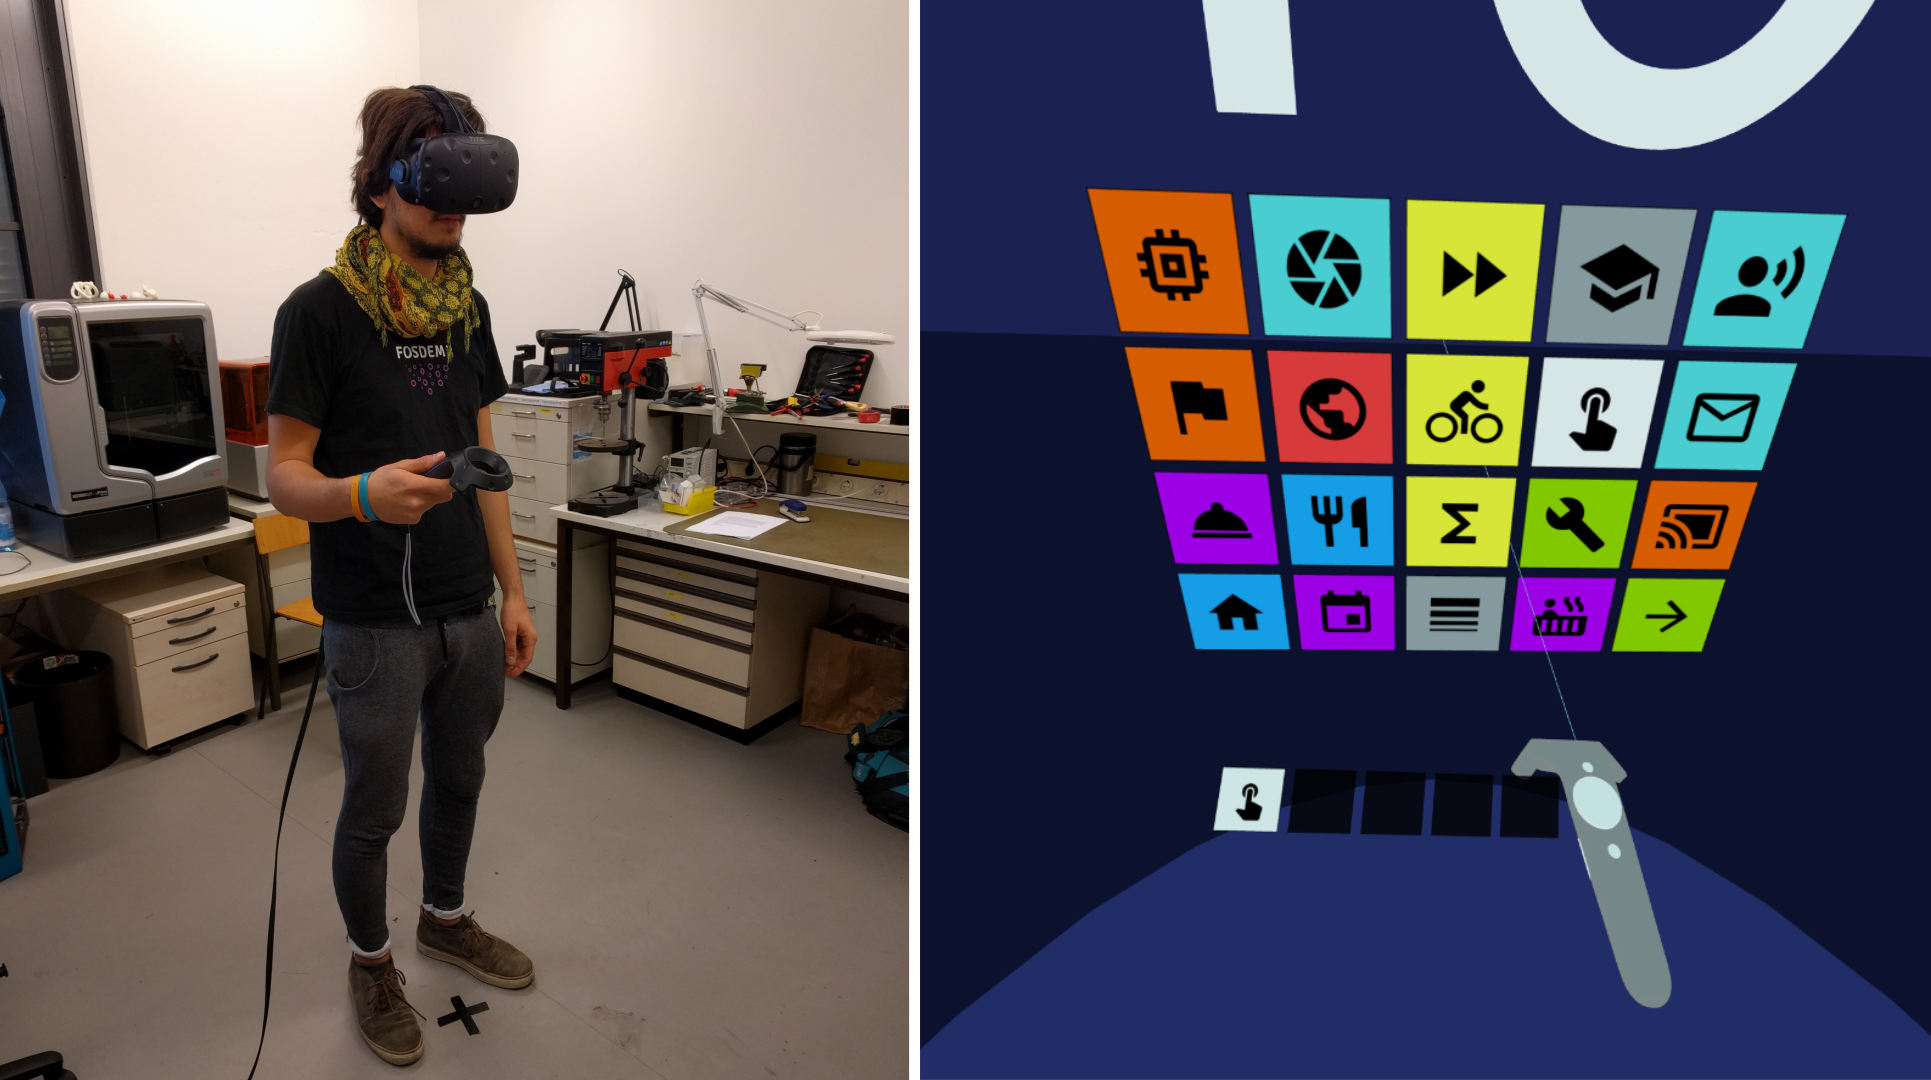
\includegraphics{participant+view.png}
  \caption{\emph{Left:} Participant standing at the designated spot in the middle of the room, wearing the Vive Headset and holding the controller. \emph{Right:} An experimental condition, as seen by the participant.}
  \label{fig:participant-view}
\end{figure}

\section{Design}
We used a within-subjects repeated measures design with three independent variables:

\begin{itemize}
  \item \emph{Interface type:} the three different interface types, \emph{Spatial}, \emph{Stacked}, and \emph{Clipped}
  \item \emph{Number of items:} 20, 50, or 150 icons
  \item \emph{Colored:} Whether all icons have the same white background, or different, colored backgrounds (from a palette of 10 colors)
\end{itemize}

The resulting 18 conditions were counterbalanced using a Latin square.

\begin{marginfigure}
  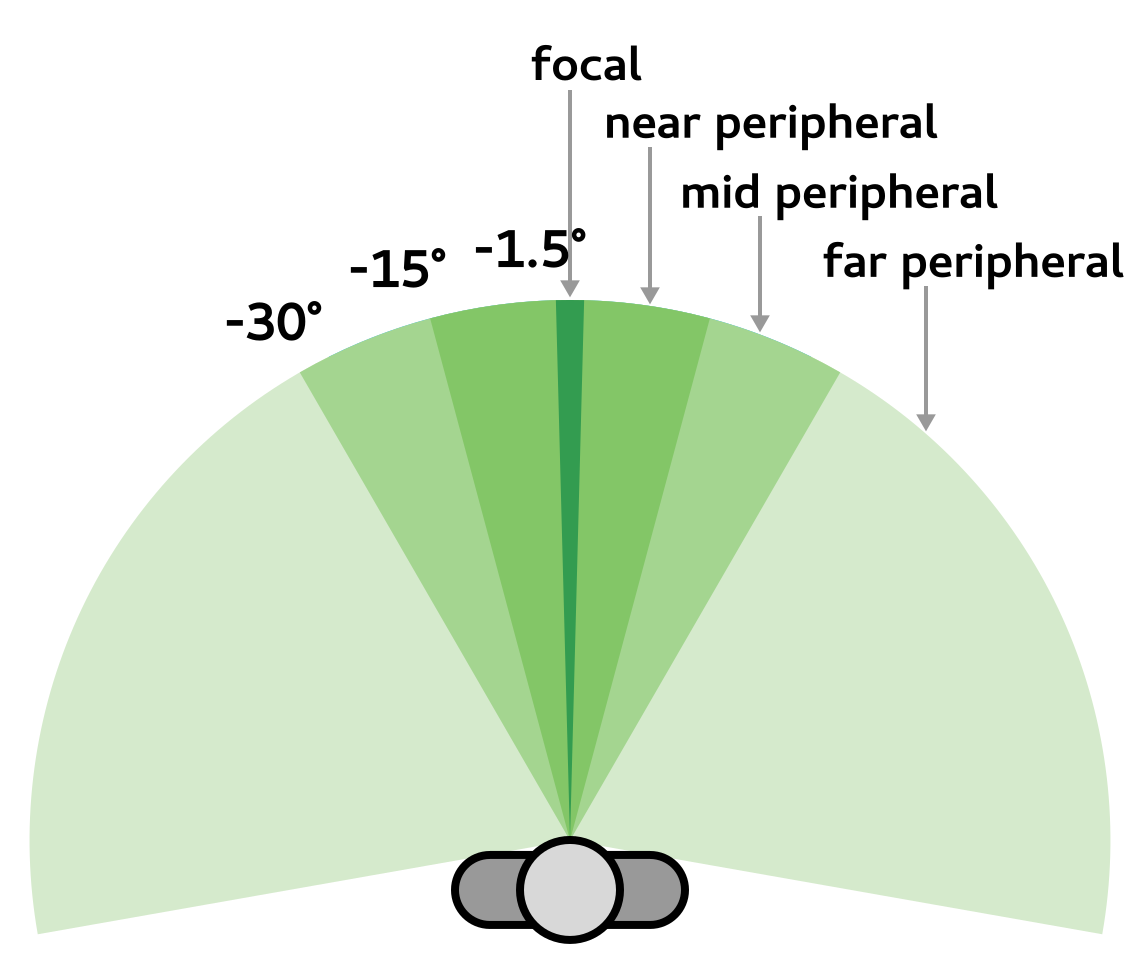
\includegraphics[width=\linewidth]{visual-field.png}
  \caption{Diagram of the human field of view}
  \label{fig:visual-field}
\end{marginfigure}

\subsection{Interface Types}
\emph{Spatial} is making use of the physical space to show all icons in a single grid. They can be navigated by simply moving one's head, and don't require additional interaction. The field of view taken up by this interface type varies from 45 to 100 degrees (see figures~\ref{fig:visual-field} and \ref{fig:fov-types}), depending on the number of icons.

\begin{figure*}[h]
  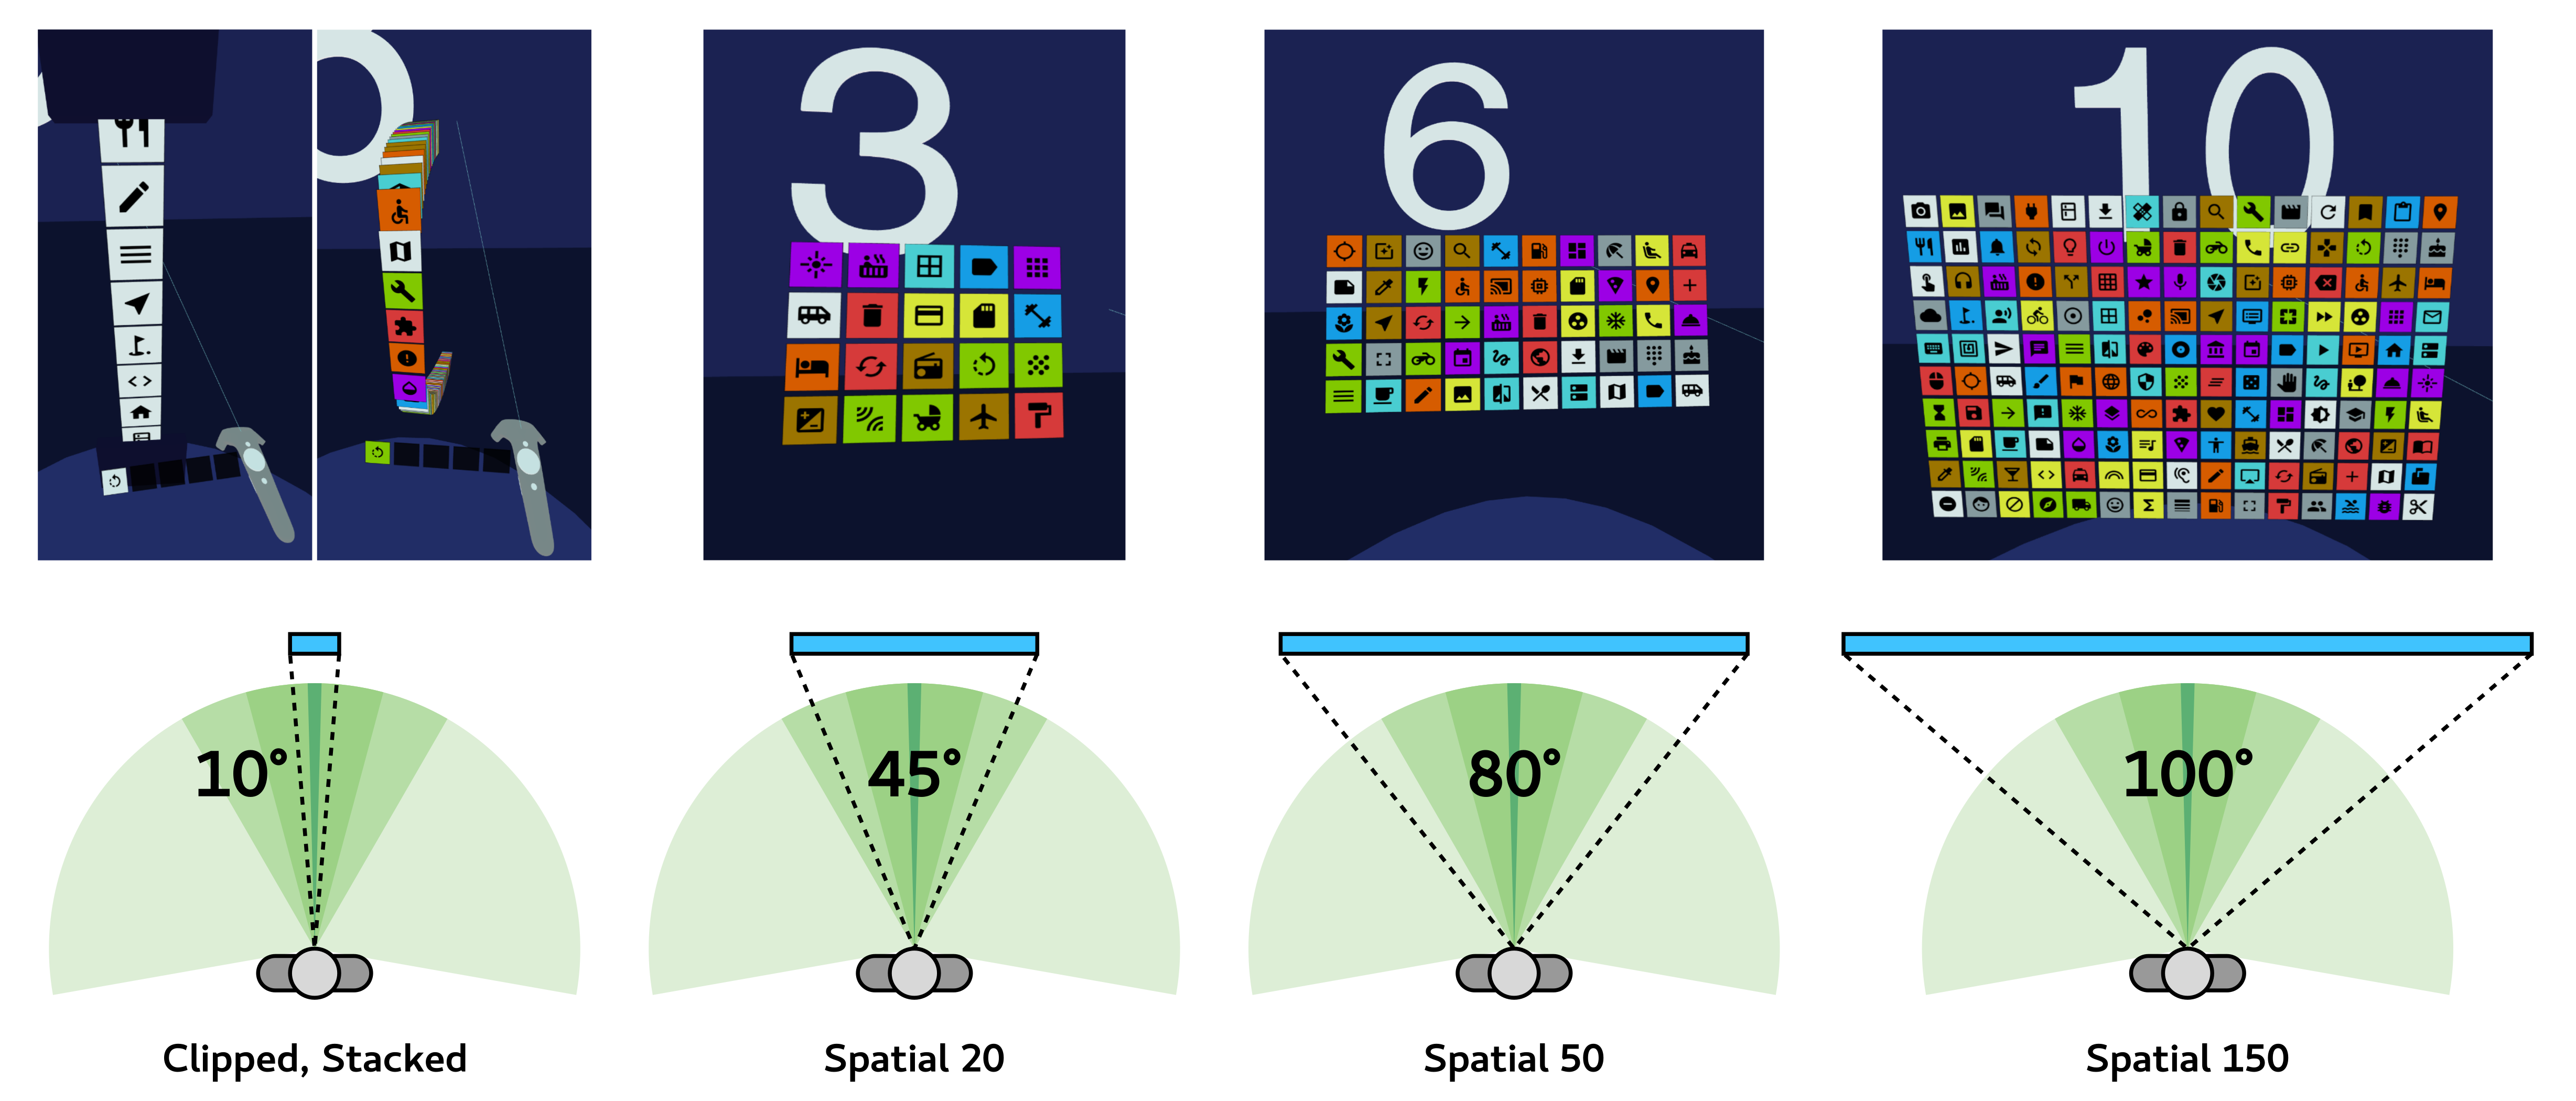
\includegraphics[width=\linewidth]{fov-types.png}
  \caption{Field of view for the different interface types}
  \label{fig:fov-types}
\end{figure*}

\emph{Stacked} is a vertically scrolling single column of icons, where overflowing elements at the top and bottom of the column stack in the z-dimension. This means that all list elements are always present in the interface and are never completely hidden. Scrolling works by pressing and holding the trigger button and moving the controller up or down. This scrolls the list continuously, following the vertical movement of the controller.

\emph{Clipped} is similar to \emph{Stacked}, except overflowing items disappear instead of stacking. The list is ``clipped'' at the top and bottom. The scrolling interaction is the same as for \emph{Stacked}.

Figure~\ref{fig:interface-types} shows how all three interface types look to participants in \textsc{vr}.

\begin{figure*}[h]
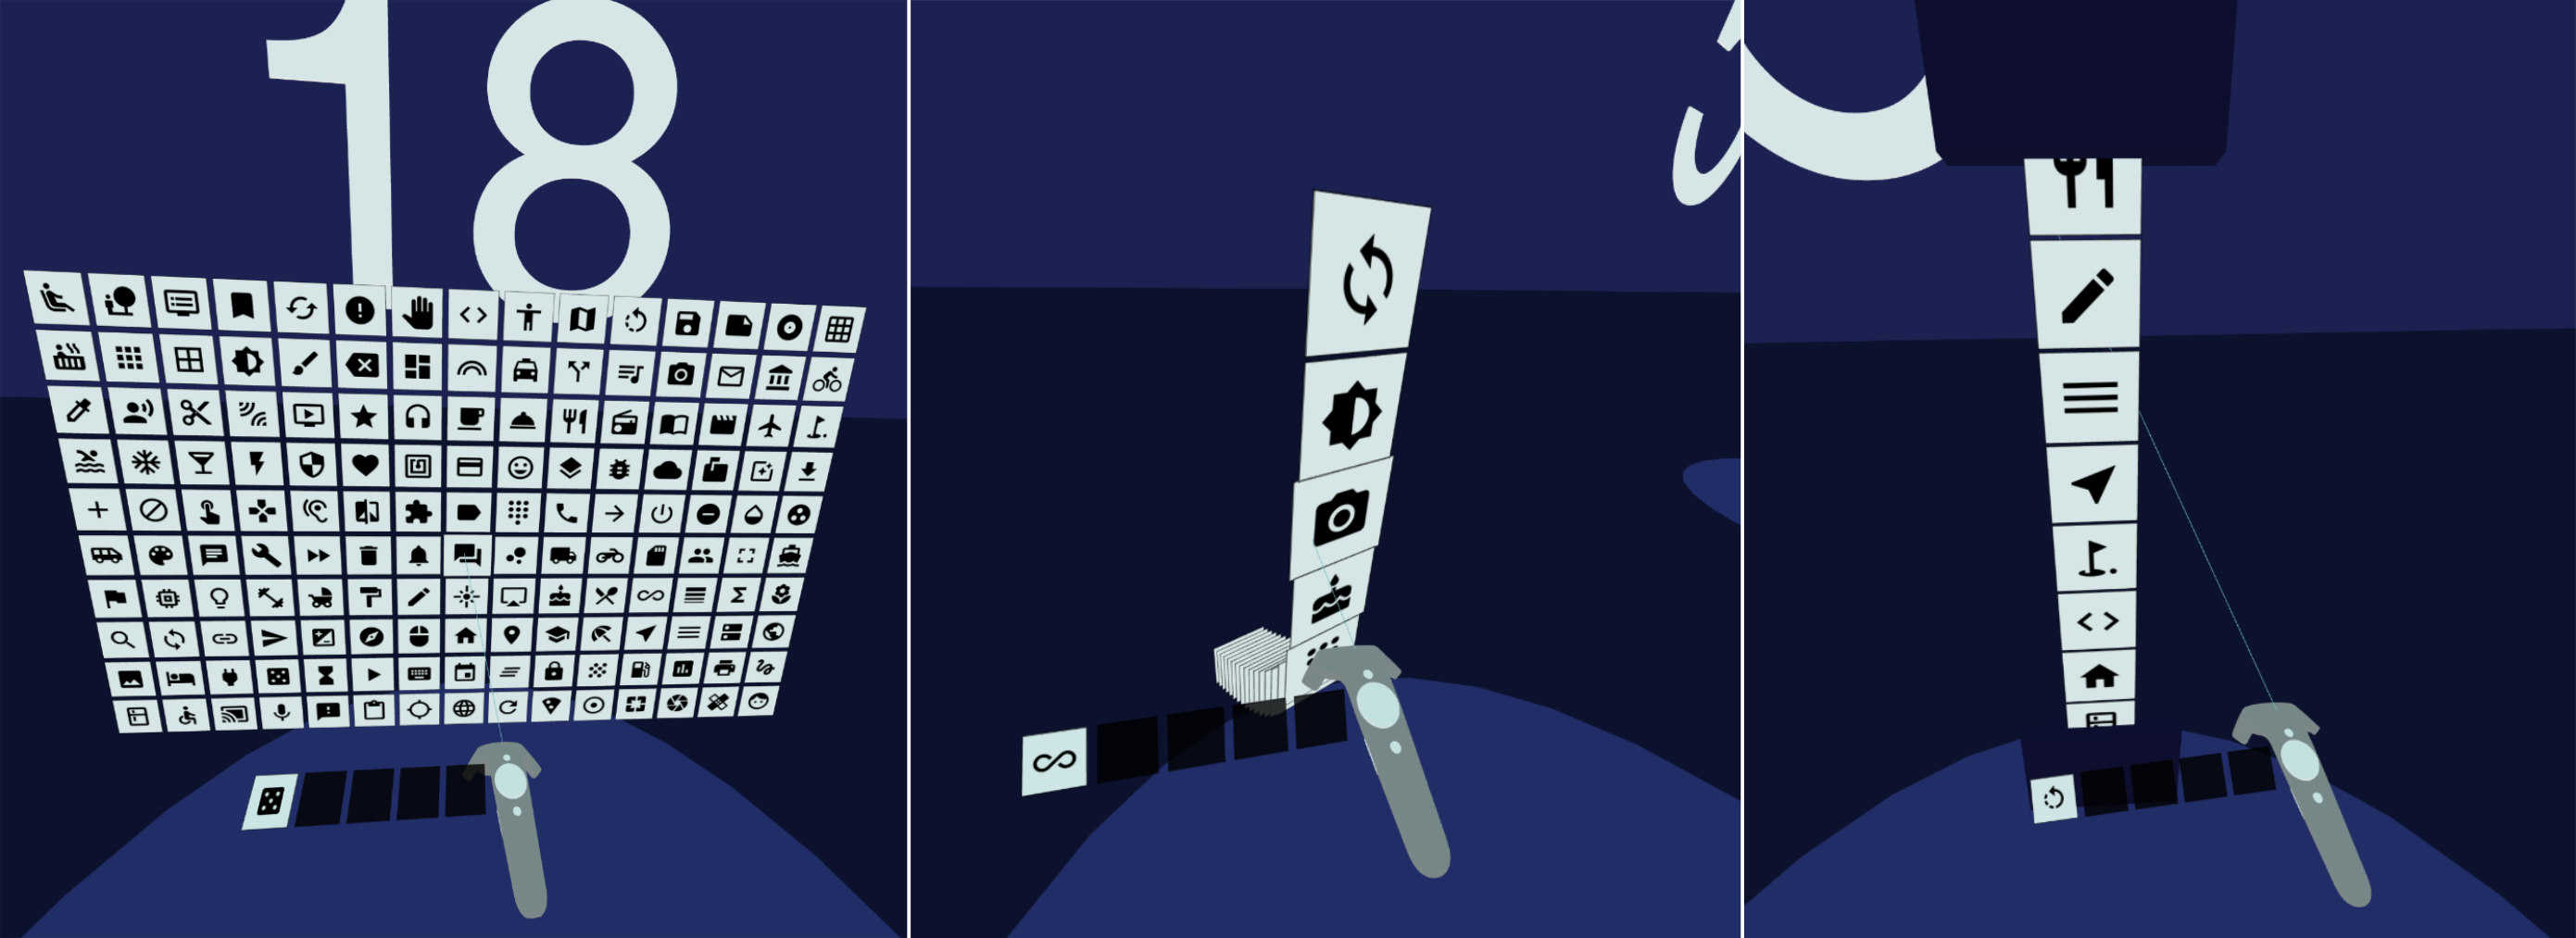
\includegraphics[width=\linewidth]{interface-types.png}
\caption{The three different interface types (left to right): \emph{Spatial}, \emph{Stacked}, and \emph{Clipped}}
\label{fig:interface-types}
\end{figure*}

\subsection{Number of Items}
The three different list sizes (20, 50, and 150) were chosen because they allowed us to test a large part of the spectrum of list sizes that realistically appear in user interfaces. We see 150 as the upper bound to the size of arbitrarily ordered, completely unstructured lists that people can handle in a practical manner. In our pilot studies we tested conditions with more items, but participants were very frustrated by the long distances they had to scroll to find icons in these conditions.

\begin{marginfigure}
  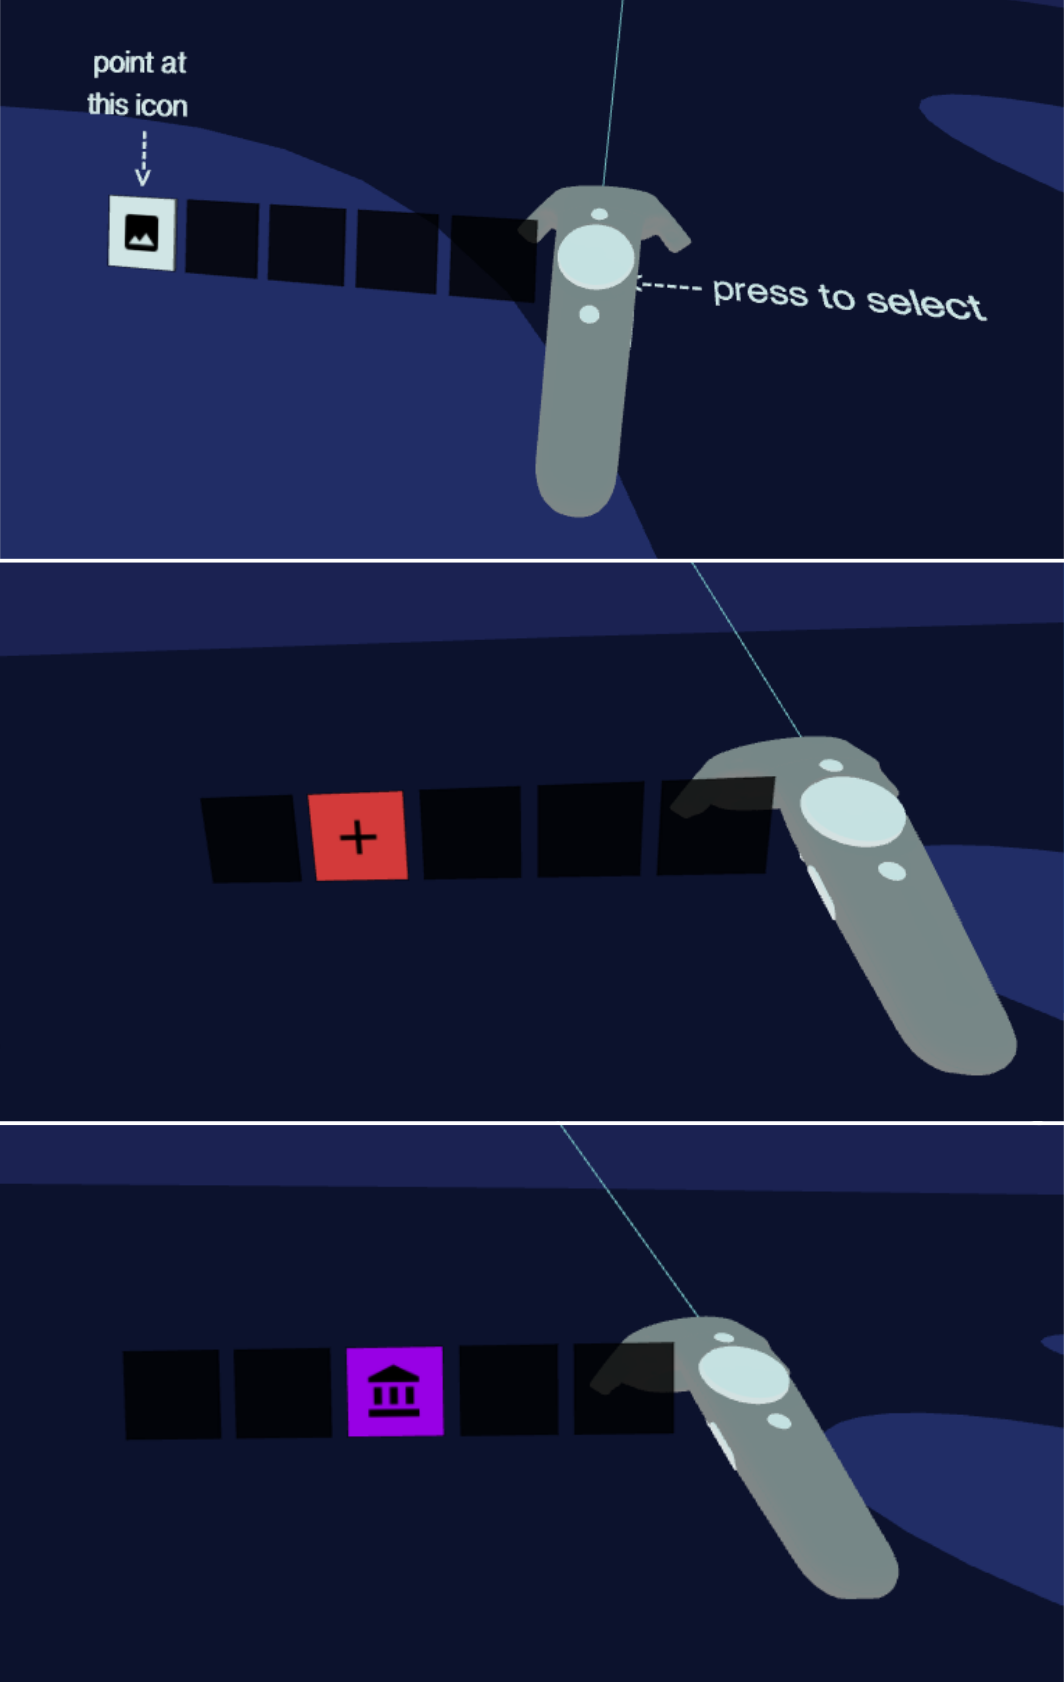
\includegraphics[width=\linewidth]{controllers.png}
  \caption{The 5 icons fixed to the left of the controller were used to guide the participants through the experiment. During each task, the current target icon was highlighted, the others were black. Selecting the target icon would reveal the next target icon on the controller, and obscure the previous one.}
  \label{fig:controllers}
\end{marginfigure}

\subsection{Colored/Monochrome}
We included the \emph{Colored} variable in order to understand the differences between \emph{Clipped} and \emph{Stacked} better. When all icons have the same background color, it is not possible to see what icons are on the ``stacked'' cards at both ends of the list. With different background colors, they can at least be differentiated when they are stacked, even though the actual icons are still obscured. We chose a palette of 10 colors that are each assigned to 10\% of the total number of icons. In addition, we also tested all conditions in a \emph{Monochrome} variant, where the background is white for all icons.

\subsection{Tasks}
The interfaces in all conditions display a number of squares with simple monochrome icons. Participants had to find specific icons, one at a time. The icon set used is a subset of the Material Design icon set used by Android and other Google products (see figure~\ref{fig:material-icons}).

\begin{figure}
  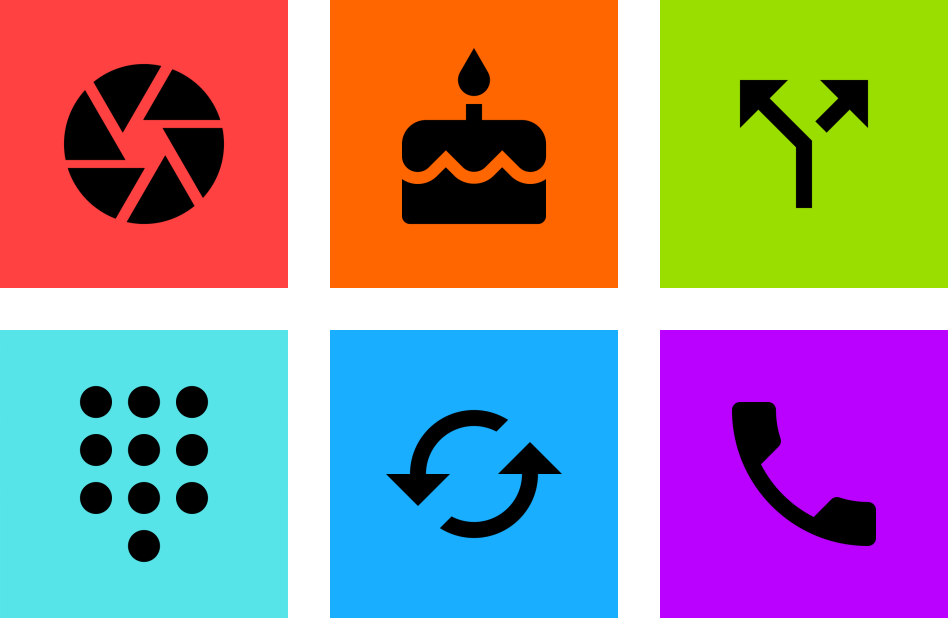
\includegraphics{material-icons.png}
  \caption{Examples of the icons used in the experiments}
  \label{fig:material-icons}
\end{figure}

\emph{Initial:} First, participants had to find 5 icons (see figure~\ref{fig:controllers}), which were pseudo-randomly distributed across the entire set (one icon per quintile). To select the icon, they had to point at it with the raycasting cursor starting from the top of their controller, and press the trigger button.

\emph{Repeat:} After finding each icon once, participants had to find the same 5 icons again, but in randomized order. Each participant had to find and select a total of 180 icons ($18$ conditions $\times$ $(5 + 5) $ icons).

\subsection{Hypotheses}
We conducted the experiment with the following hypotheses in mind:

\begin{enumerate}[label=H\arabic*. , wide=0.5em,  leftmargin=*]
  \item \emph{Spatial} outperforms \emph{Clipped} and \emph{Stacked}: \emph{Spatial} allows participants to explore the entire set of icons by simply turning their heads, rather than using the controller, so we assumed it would this condition would be the fastest.
  \item \emph{Repeat} outperforms \emph{Initial}: During the second round of each condition, participants only had to find icons that they'd found before, which we assumed would be faster due to spatial memory \cite{scarr2013supporting}.
  \begin{enumerate}[label=H2.\arabic*. , wide=0.5em,  leftmargin=*]
    \item \emph{Clipped} and \emph{Stacked} perform similarly for \emph{Initial}: Due to the similarities in structure and interaction, we assumed that there should be no difference between them in this case.
    \item \emph{Stacked} outperforms \emph{Clipped} for \emph{Repeat Colored}: Since \emph{Stacked} does not hide elements completely, but stacks them in space, we assumed participants would have a clearer sense of their position and find them more easily the second time.
  \end{enumerate}
  \item \emph{Colored} outperforms \emph{Monochrome}: Since searching for a \emph{Colored} icon requires only looking at icons that have the correct color, we assumed this would be faster than searching through all icons.
\end{enumerate}

\section{Procedure}
Participants were given a demographic questionnaire, and then introduced to the \textsc{vr} setup. They put on the headset and were handed the controller. They then received instructions for how to use the interfaces in the experiment from a short tutorial in \textsc{vr} (see figure~\ref{fig:tutorials}). The tutorial consists of two parts.
In the first part the participants were shown how to select icons using the right controller's raycasting cursor.

\begin{figure*}[h]
  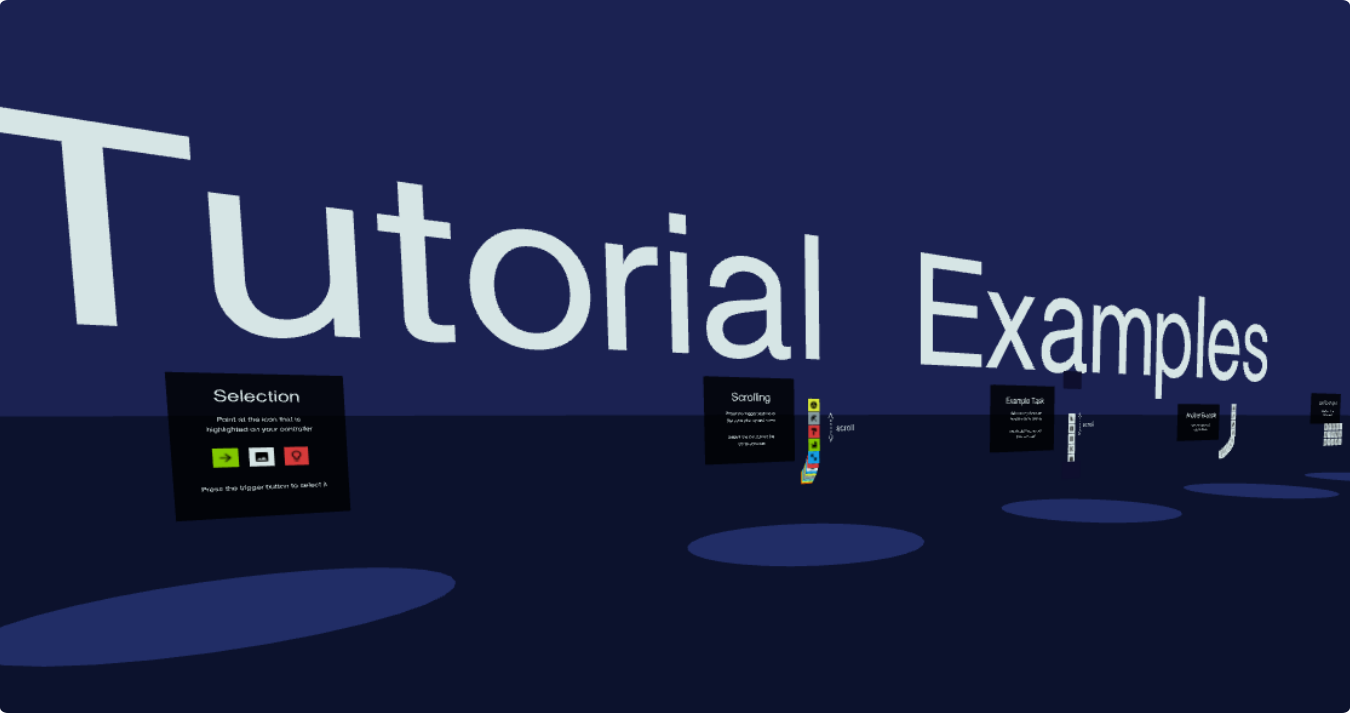
\includegraphics[width=\linewidth]{tutorials.png}
  \caption{The five initial steps of the experiment, including 2 tutorial and 3 example steps.}
  \label{fig:tutorials}
\end{figure*}

In the second part they were shown how to scroll in \emph{Clipped} and \emph{Stacked} interfaces, by keeping the trigger button pressed and moving the controller vertically.
Participants were told to perform the tasks \emph{as quickly as possible without making any errors}.

After being introduced to the basic interactions, participants got 3 example conditions (one for each interface type). This allowed them to learn the mechanics and get comfortable with the different interfaces before the actual experiment.

Then they performed the tasks for all 18 conditions, counterbalanced using a Latin square. After each condition, they answered a questionnaire (inside the \textsc{vr} environment) with four qualitative statements assessing their experience with a given condition. Figure~\ref{fig:questionnaire} is a screenshot of what this questionnaire looked like to participants. They rated each of the statements by ``clicking'' one of the 7 squares using the same raycasting pointer mechanic used during the experimental conditions. Participants rated each of the statements on a 7-point Likert scale (1 = not true at all, 7 = very true).

\begin{marginfigure}
  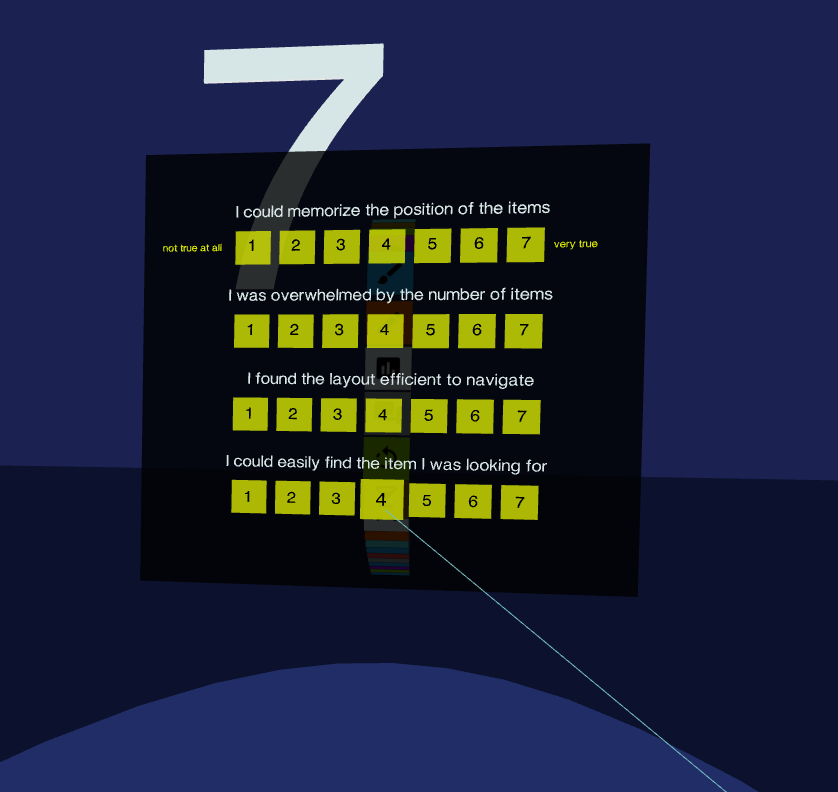
\includegraphics{questionnaire.png}
  \caption{The qualitiative questionnaire participants filled in after each of the 18 conditions.}
  \label{fig:questionnaire}
\end{marginfigure}

These are the four statements:

\begin{enumerate}[label=\arabic*. , wide=0.5em,  leftmargin=*]
  \item I could memorize the position of the items.
  \item I was overwhelmed by the number of items.
  \item I found the layout efficient to navigate.
  \item I could easily find the item I was looking for.
\end{enumerate}


After the experiment, which lasted about 45 minutes, participants were given a questionnaire rating the three interface types (both \emph{Colored} and \emph{Monochrome}) on a 7-point Likert scale (1 = very negatively, 7 = very positively).

\section{Data Collection}
For each condition, we logged the time participants took to select each icon. We also logged selection errors (selection of non-target icons), scroll distances for \emph{Clipped} and \emph{Stacked} conditions, and controller movement in the room throughout the experiments.

For each individual icon that had to be selected during the experiment, we logged the following variables:

\begin{itemize}
  \item The time it took to select select in milliseconds
  \item The scrolled distance in meters (only for conditions that require scrolling)
  \item Controller movement in meters
  \item Selection errors (selection of non-target icons)
\end{itemize}


Of these variables, only selection time was really necessary for our hypotheses, but we chose to log the additional variables to get a more complete picture and find potential problems in our data more easily.


%----------------------------------------------------------------------------------------
%	RESULTS
%----------------------------------------------------------------------------------------

\chapter{Results}
\label{ch:results}

This chapter presents the qualitative and quantitive results of our study, including the metrics measured during the experiment, the \textsc{vr} questionnaires after each condition, and the questionnaire at the end of the experiment.

\section{Quantitative Results}
Of the quantitative variables measured during the experiment, \emph{Selection Time} is the most important. It is measured as the time interval between when the target icon is shown on the controller and when it is selected. All our main hypotheses are about quantitative performance, which is assessed using \emph{Selection Time}. Figure~\ref{fig:all-durations-chart} gives an overview of our results for the different interface types.

\begin{figure*}[h]
  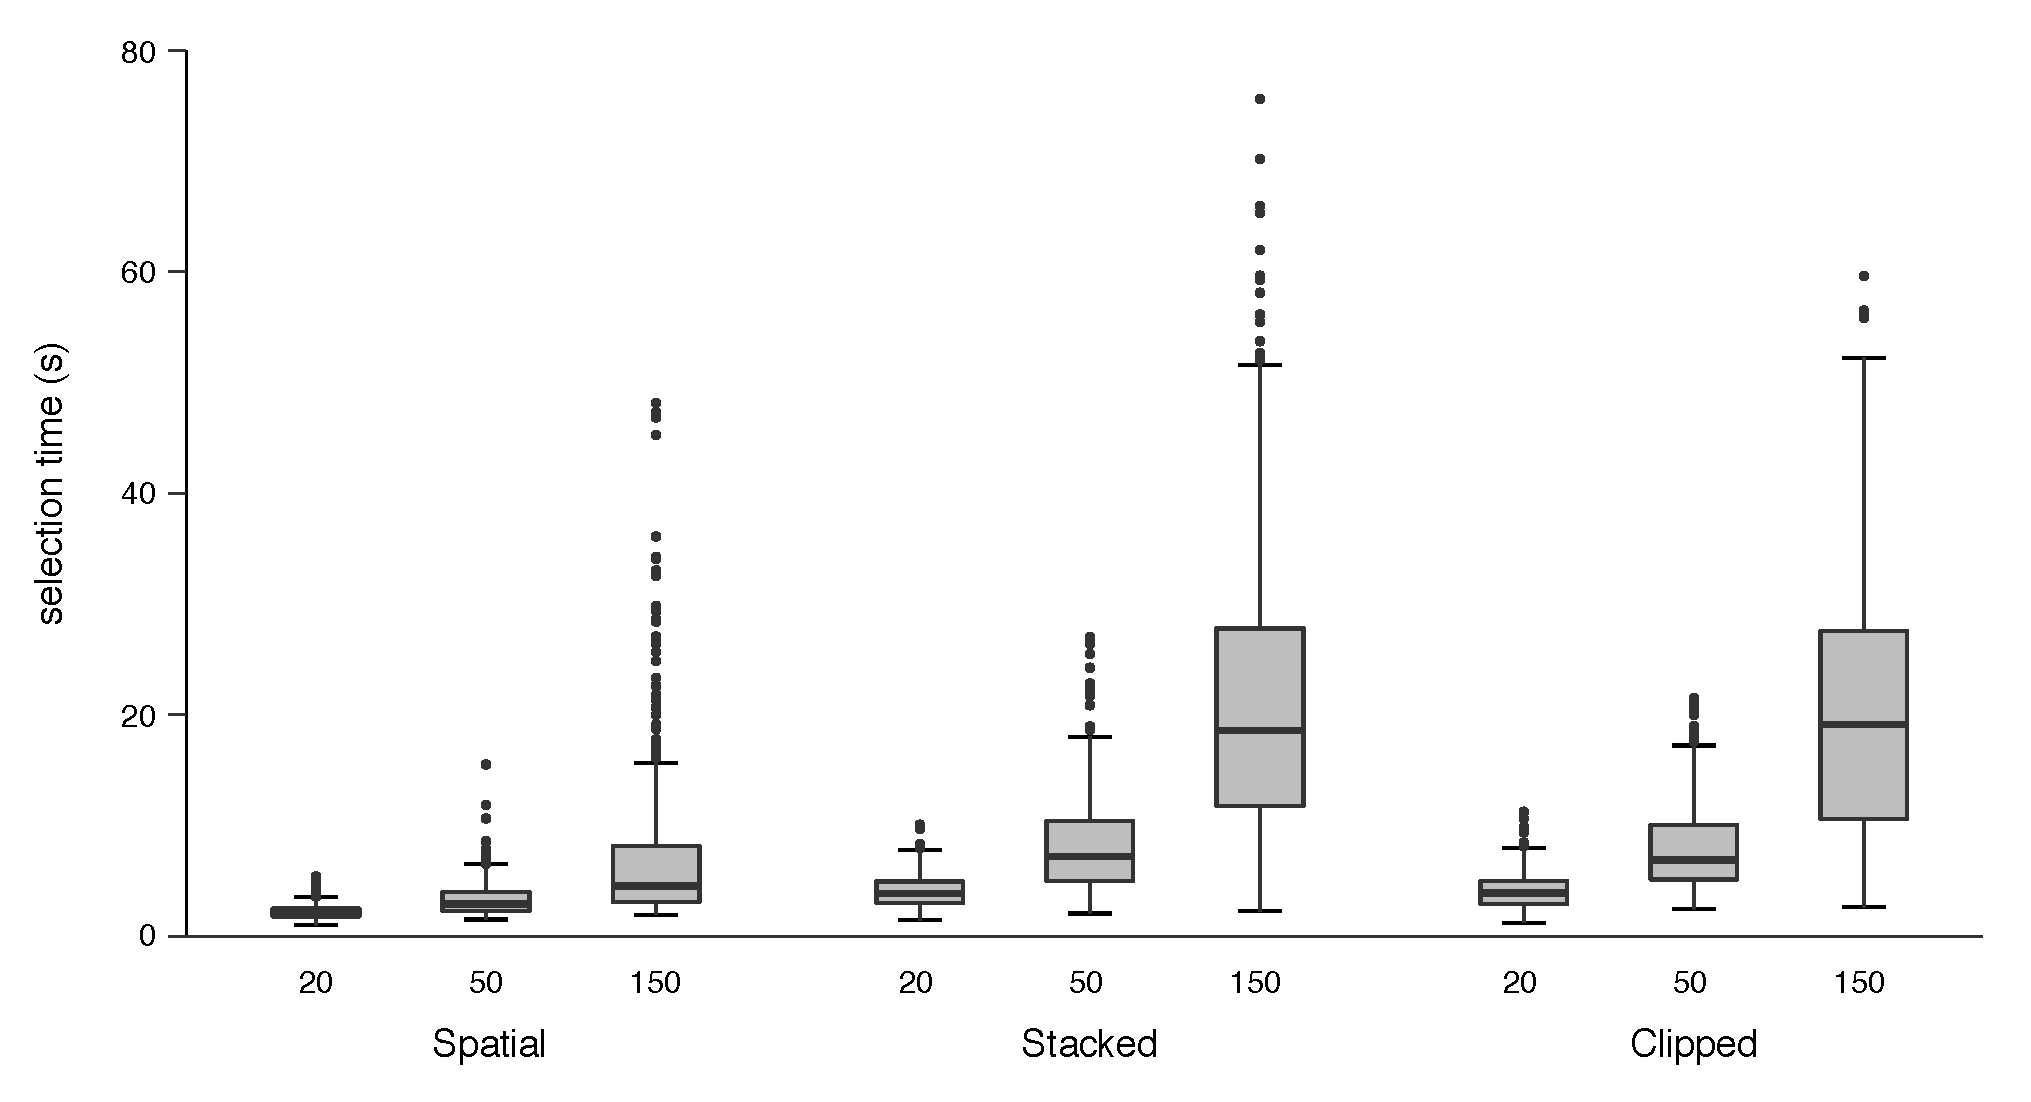
\includegraphics[width=\linewidth]{all-durations.pdf}
  \caption{Selection time for all interface types and list sizes}
  \label{fig:all-durations-chart}
\end{figure*}

\subsection{Summary of Results}
Our primary hypotheses were that in \emph{Spatial} conditions, it would take less time to select icons (H1), and that finding icons the second time would be faster than the first time (H2). Both of these were confirmed. In addition, we hypothesized that \emph{Clipped} and \emph{Stacked} should perform similarly for the initial finding of icons (H2.1), which was confirmed, and that \emph{Stacked} should outperform \emph{Clipped} in \emph{Repeat Colored} conditions (H2.2), which was not confirmed.
Lastly, we theorized that finding \emph{Colored} icons would be faster than \emph{Monochrome} ones (H3), which was confirmed.

\subsection{Data Processing}
The data recorded by the experimental software was saved in \textsc{csv} files, aggregated, and cleaned of invalid data points in Excel. 35 out of 3600 trials had 1 or 2 errors, which means that 99.03\% were valid. Then we computed the average and standard deviation for all conditions. We did not find any systematic error across conditions.

After removing trials with errors, 44 trials were excluded for having an average larger or smaller than 3 standard deviations than the average of the specific condition. This left us with 3521 (97.81\%) valid trials. This is the data we used in our analysis, which we performed using the open source statistics package \textsc{jasp}\footnote{JASP: Open Source Statistical Software (https://jasp-stats.org)}.

\subsection{H1: Spatial outperforms Stacked and Clipped}
We hypothesized that the selection time would be significantly shorter for \emph{Spatial} conditions compared to both \emph{Stacked} and \emph{Clipped} conditions. Our results confirmed that this is true in both cases (see figure~\ref{fig:duration-types}). We performed an individual one-way \textsc{anova} ($\alpha = .05$) on the dependent variable selection time. We found a significant main effect from the interface type ($F(5,3515) = 98.92, p < .001$).
A Tukey post-hoc test revealed that the selection time in \emph{Spatial} conditions was significantly lower than in both \emph{Stacked} ($p < .001$) and \emph{Clipped} ($p < .001$) conditions. The mean selection time for \emph{Spatial} conditions was $4.32 s$ ($SD = 5.05 s$), for \emph{Stacked} conditions it was $11.25 s$ ($SD = 10.89 s$), and for \emph{Clipped} $10.92 s$ ($SD = 10.09 s$).

\begin{marginfigure}
  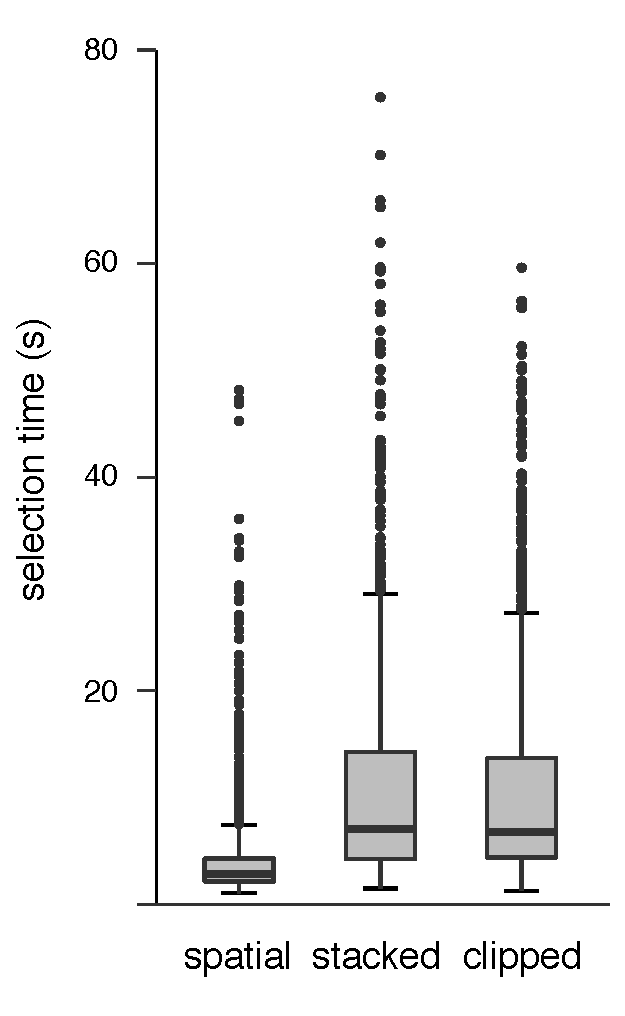
\includegraphics[width=\linewidth]{duration-types.pdf}
  \caption{Selection time for the three different experiment types}
  \label{fig:duration-types}
\end{marginfigure}

\subsection{H2: Repeat outperforms Initial}
Our second hypothesis was that on average, selections should be faster for icons that have already been found previously (\emph{Repeat}), compared to icons the participants have not seen before in a given condition (\emph{Initial}). This was confirmed by our results. We performed an individual one-way \textsc{anova} ($F(\alpha = .05$) on the dependent variable selection time and found a significant main effect from whether conditions were \emph{Initial} or Repeat ($F(1,3519) = 47.27, p < .001$).
A Tukey post-hoc test revealed that \emph{Repeat} icons were found significantly faster than \emph{Initial} ones ($p < .001$). The mean selection time for \emph{Initial} icons was $9.94 s$ ($SD = 10.49 s$), while for \emph{Repeat} icons it was $7.74 s$ ($SD = 8.47 s$).

\subsection{H2.1: Clipped and Stacked perform similarly for Initial}
We hypothesized that for \emph{Initial} icons there should not be any performance difference between \emph{Stacked} and Clipped, since participants had not scrolled the list yet and could therefore not rely on spatial memory and the partially visible icons to find their target icons more quickly. We performed an individual one-way \textsc{anova} ($F(2,1774) = 159.6, \alpha = .05$) on the dependent variable selection time using only \emph{Initial} trials, and found a significant main effect from the interface type ($F(2,1774) = 139.9, p < .001$).
A Tukey post-hoc test did not reveal a significant difference between \emph{Stacked} and \emph{Clipped} ($p = .631$). The mean selection time for \emph{Stacked} icons was $10.17 s$ ($SD = 9.81 s$), while for \emph{Clipped} icons it was $9.75 s$ ($SD = 9.00 s$).

\subsection{H2.2: Stacked outperforms Clipped for Repeat Colored}
The reason why we included \emph{Colored} conditions was because we assumed this could impact the difference in performance between \emph{Stacked} and \emph{Clipped}. When all icons have the same white background, they are not distinguishable at all while stacked. When the backgrounds are colored, it's possible to recognize stacked icons to a limited degree by their color, and see patterns and sequences of colors even if the icons are not directly visible.

\begin{marginfigure}
  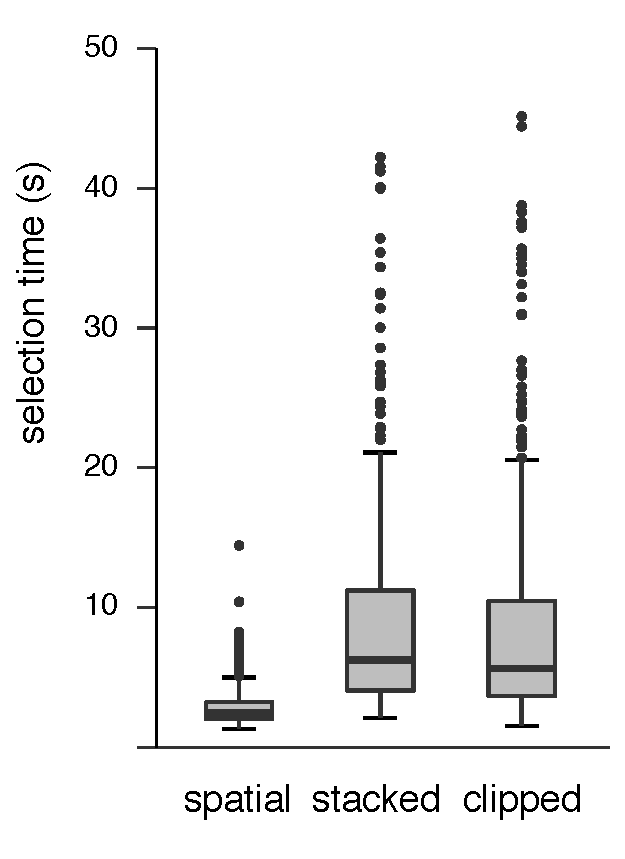
\includegraphics[width=\linewidth]{repeat-color.pdf}
  \caption{Selection time for different experiment types (only \emph{Repeat Color} icons)}
  \label{fig:repeat-color}
\end{marginfigure}

Our assumption was that this would result in better performance for \emph{Stacked} compared to \emph{Clipped} in \emph{Repeat Colored} conditions, but this was not confirmed. We performed an individual one-way \textsc{anova} ($\alpha = .05$) on the dependent variable selection time using only \emph{Repeat} trials (see figure~\ref{fig:repeat-color}) and found a significant main effect ($F(2,882) = 81.92, p < .001$) from interface type.
However, a Tukey post-hoc test revealed no significant difference between \emph{Stacked} and \emph{Clipped} for \emph{Repeat Colored} icons ($p = .95$). The mean selection time for \emph{Stacked} icons was $9.45 s$ ($SD = 8.11 s$), while for \emph{Clipped} icons it was $9.27 s$ ($SD = 8.90 s$).

\subsection{H3: Colored outperforms Monochrome}
Our last hypothesis was that \emph{Colored} conditions should perform better than \emph{Monochrome} ones on average, because the colors help reduce the number of icons that have to be scanned to only the ones with the right color. This was confirmed by an individual one-way \textsc{anova} ($\alpha = .05$) on the dependent variable selection time, which showed a significant main effect from color ($F(1,3519) = 30.79, p < .001$).
A Tukey post-hoc test revealed that the performance of \emph{Colored} icons was significantly better than \emph{Monochrome} ones ($p < .001$). The mean selection time for \emph{Colored} icons was $7.94 s$ ($SD = 8.09 s$), while for \emph{Monochrome} icons it was $9.72 s$ ($SD = 10.81 s$). Such a significant result is interesting because we had assumed that colors could potentially be distracting, and therefore impact performance negatively.

\section{Qualitative Results}

We collected qualitative data about the user experience of our prototypes using two questionnaires: One per-condition questionnaire that participants filled in inside the \textsc{vr} environment, right after each condition, and a paper questionnaire after the experiment was concluded. The qualitative data confirms the findings of the quantitative study for the most part, as participants preferred \emph{Spatial} conditions over \emph{Stacked} and \emph{Clipped} ones, and \emph{Colored} ones over \emph{Monochrome}. However, there are also some interesting differences, such as the preference for \emph{Stacked} over \emph{Clipped} (even though there is no measurable quantitative performance difference).

\subsection{Post-Condition Questionnaire}
After each of the 18 conditions, participants rated four qualitative statements assessing their experience with a given condition on a 7-point Likert scale. For the most part, the results from these questionnaires match our findings from the quantitative data.

\begin{figure}
  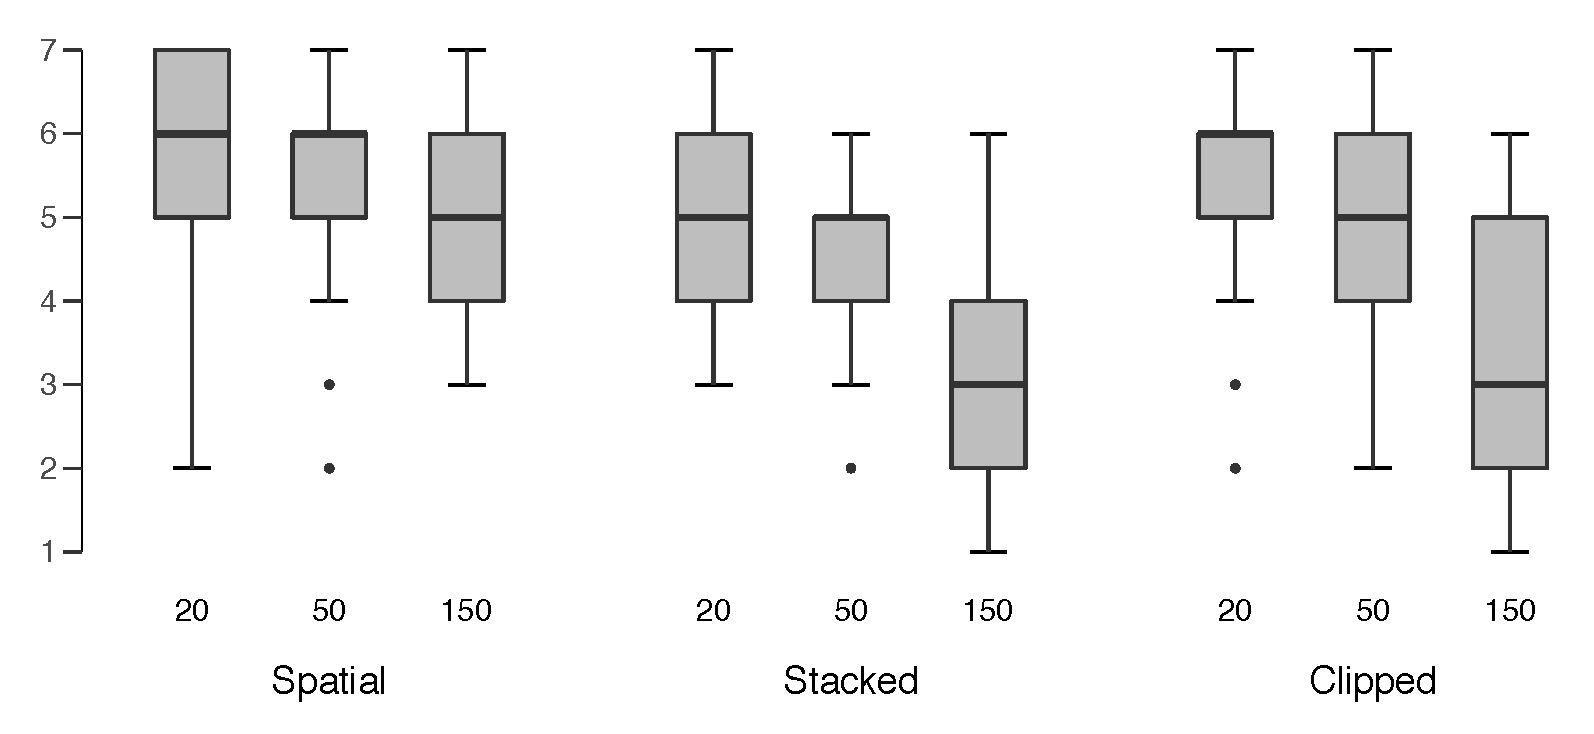
\includegraphics{postcon-memorize.pdf}
  \caption{Responses to ``I could memorize the position of the items'' split by interface type and number of icons (Likert scale, 1=not true at all, 7=very true)}
  \label{fig:memorize}
\end{figure}

\emph{``I could memorize the position of the items''}:
An individual one-way \textsc{anova} ($\alpha = .05$) on the dependent variable rating shows a significant main effect from interface type ($F(2,345) = 24.5, p < .001$), number of icons ($F(2,345) = 46, p < .001$), but not color ($F(1,345) = 0.029, p = .86$).

A Tukey post-hoc test revealed that icon positions in \emph{Spatial} conditions were seen as significantly easier to memorize than in \emph{Stacked} ($p < .001$) and \emph{Clipped} ($p < .001$), while there was no signifcant difference between \emph{Stacked} and \emph{Clipped} ($p = .61$). We also found a significant differences between all sizes of the conditions, between 20 and 50 ($p = .049$), 20 and 150 ($p < .001$), and 50 and 150 ($p < .001$). This shows that participants found \emph{Spatial} conditions significantly easier to memorize, but didn't perceive a difference between \emph{Colored}/\emph{Monochrome} and \emph{Stacked}/\emph{Clipped} conditions. The number of icons was also a significant factor, especially for \emph{Stacked} and \emph{Clipped}, as figure~\ref{fig:memorize} shows.

\emph{``I was overwhelmed by the number of items''}:
An individual one-way \textsc{anova} ($\alpha = .05$) on the dependent variable rating shows a significant main effect from interface type ($F(2,345) = 7.97, p < .001$), number of icons ($F(2,345) = 192.78, p < .001$), but not color ($F(1,345) = 3.03, p = .083$).

A Tukey post-hoc test revealed that participants found \emph{Spatial} conditions less overwhelming than \emph{Stacked} ($p < .001$), but there was no difference between \emph{Spatial} and \emph{Clipped} ($p = .64$). \emph{Clipped} was rated to be less overwhelming than \emph{Stacked} ($p = .024$). We also found a significant differences between all sizes of the conditions, between 20 and 50 ($p < .001$), 20 and 150 ($p < .001$), and 50 and 150 ($p < .001$). The fact that participants found \emph{Spatial} conditions least overwhelming is interesting, as we had assumed that especially in larger conditions, showing all elements at once would be overwhelming. As figure~\ref{fig:overwhelmed} shows this is not the case.

\begin{figure}
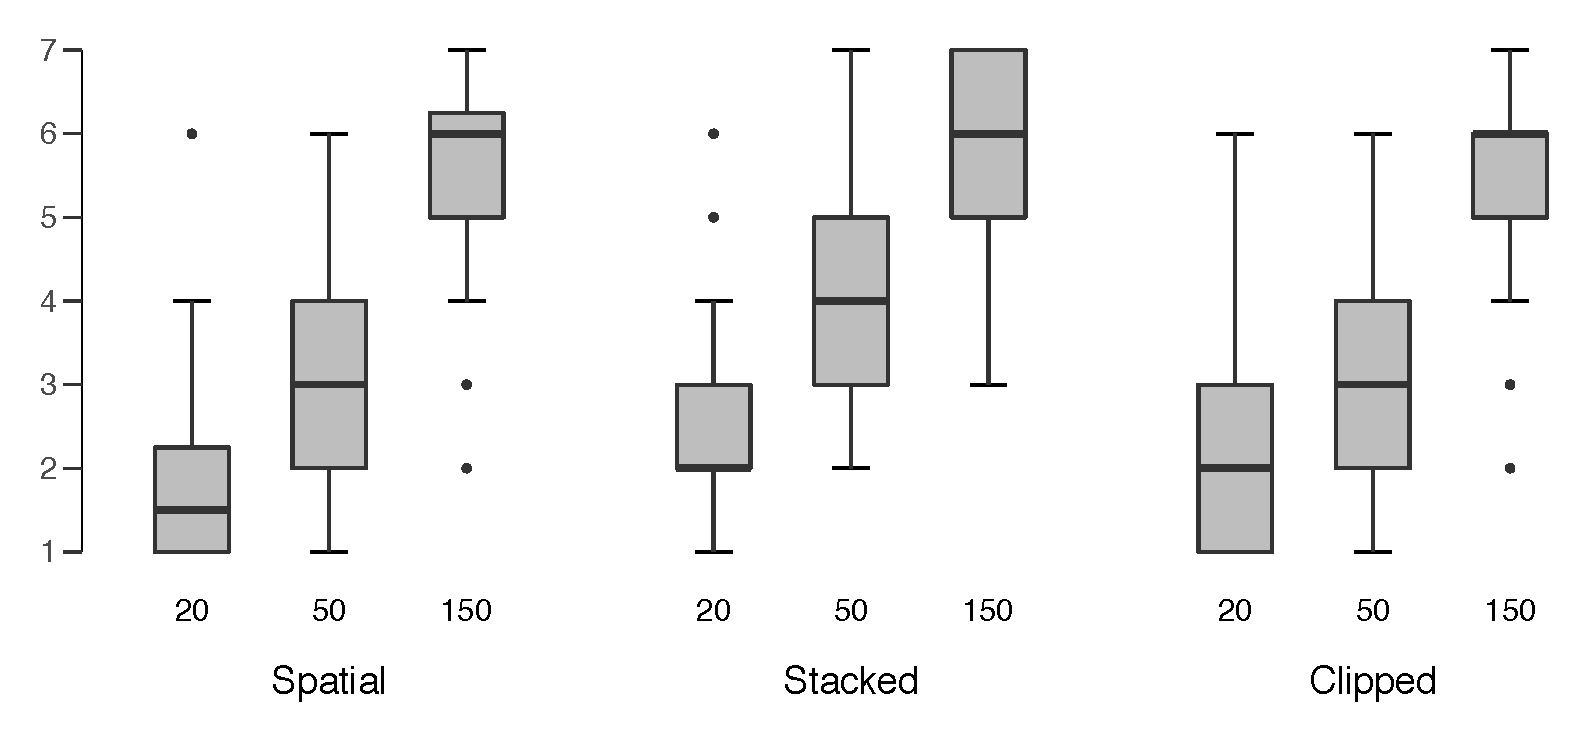
\includegraphics{postcon-overwhelmed.pdf}
\caption{Responses to ``I was overwhelmed by the number of items'' split by interface type and number of icons (Likert scale, 1=not true at all, 7=very true)}
\label{fig:overwhelmed}
\end{figure}

\emph{``I found the layout efficient to navigate''}
An individual one-way \textsc{anova} ($\alpha = .05$) on the dependent variable rating shows a significant main effect from interface type ($F(2,345) = 31.12, p < .001$), number of icons ($F(2,345) = 51.63, p < .001$), and color ($F(1,345) = 7.88, p = .005$).

A Tukey post-hoc test revealed that \emph{Spatial} conditions were seen as significantly more efficient to navigate than in \emph{Stacked} ($p < .001$) and \emph{Clipped} ($p < .001$), while there was no signifcant difference between \emph{Stacked} and \emph{Clipped} ($p = 1$). \emph{Colored} conditions were rated more efficient than \emph{Monochrome} ones ($p = .005$). We also found a significant differences between all sizes of the conditions, between 20 and 50 ($p = .006$), 20 and 150 ($p < .001$), and 50 and 150 ($p < .001$). This shows that participants found \emph{Spatial} conditions significantly more efficient to navigate, but didn't perceive a difference between \emph{Stacked} and \emph{Clipped} conditions. The number of icons was also a significant factor, as is clearly visible in figure~\ref{fig:efficient}.

\begin{figure}
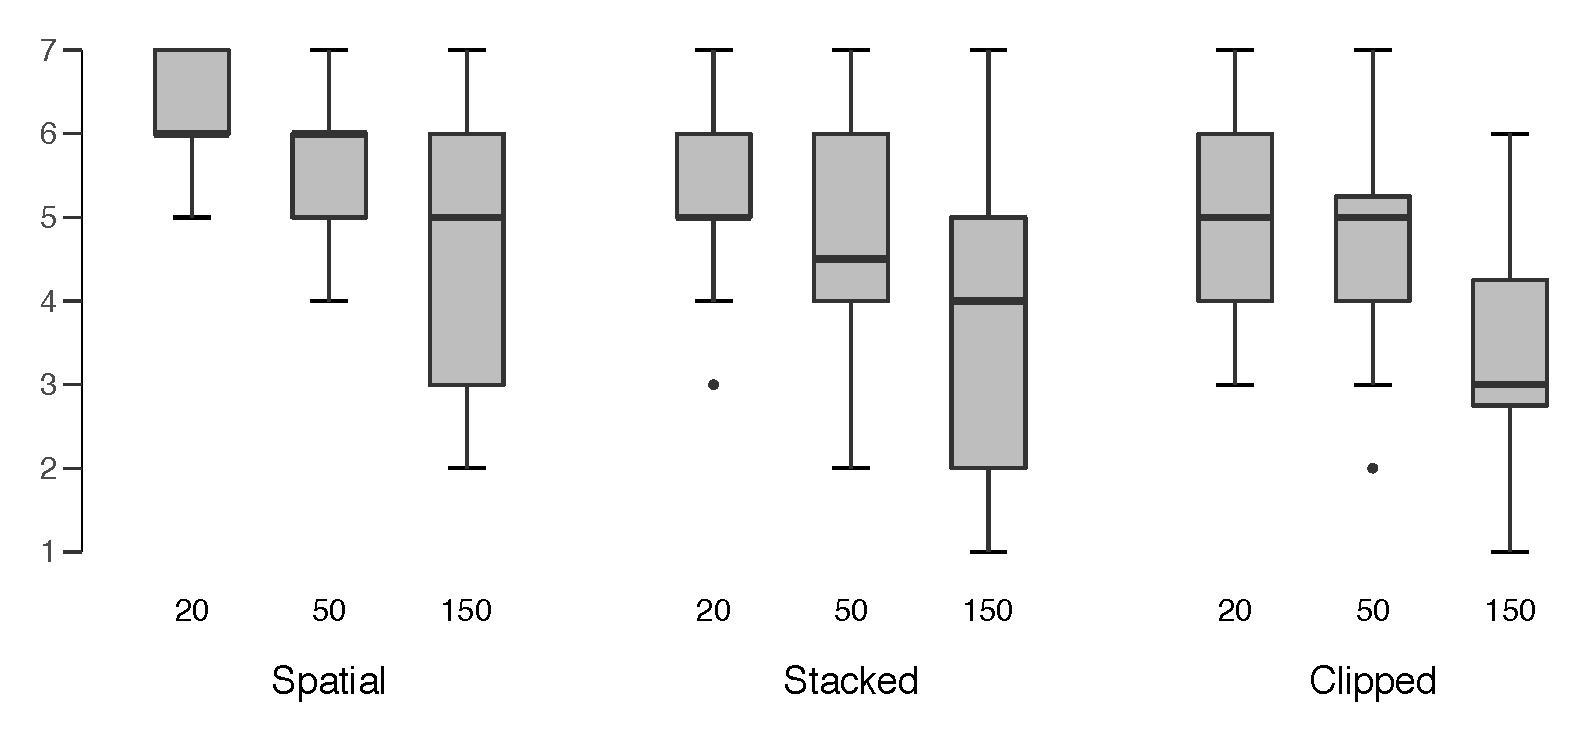
\includegraphics{postcon-efficient.pdf}
\caption{Responses to ``I found the layout efficient to navigate'' split by interface type and number of icons (Likert scale, 1=not true at all, 7=very true)}
\label{fig:efficient}
\end{figure}

\emph{``I could easily find the item I was looking for''}
An individual one-way \textsc{anova} ($\alpha = .05$) on the dependent variable rating shows a significant main effect from interface type ($F(2,345) = 21.6, p < .001$), number of icons ($F(2,345) = 131.35, p < .001$), and color ($F(1,345) = 8.24, p = .004$).

A Tukey post-hoc test revealed that icons in \emph{Spatial} conditions were seen as significantly more easy to find than in \emph{Stacked} ($p < .001$) and \emph{Clipped} ($p < .001$), while there was no signifcant difference between \emph{Stacked} and \emph{Clipped} ($p = .72$). \emph{Colored} conditions were rated more highly than \emph{Monochrome} ones ($p = .004$). We also found a significant differences between all sizes of the conditions, between 20 and 50 ($p < .001$), 20 and 150 ($p < .001$), and 50 and 150 ($p < .001$). This shows that participants found icons easiest to find in \emph{Spatial} and \emph{Colored} conditions, but didn't perceive a difference between \emph{Stacked} and \emph{Clipped} conditions (see figure~\ref{fig:easyfind}). The number of icons was also a significant factor.

\begin{figure}
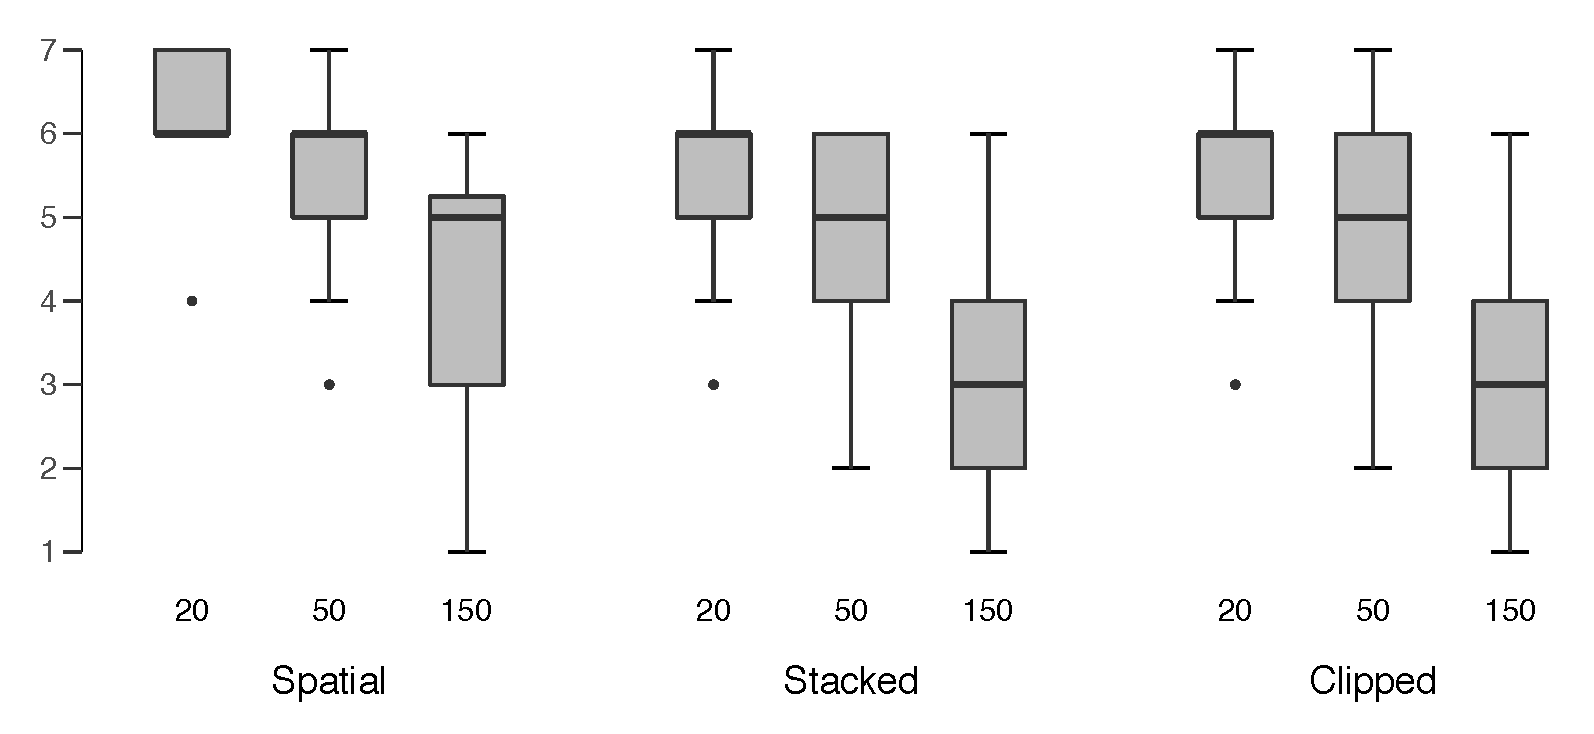
\includegraphics{postcon-easy.pdf}
\caption{Responses to ``I could easily find the item I was looking for'' split by interface type and number of icons (Likert scale, 1=not true at all, 7=very true)}
\label{fig:easyfind}
\end{figure}


\subsection{Post-Experiment Questionnaire}
After participants completed the experiment, they filled in a short paper questionnaire assessing their experience with the different interfaces. For each combination of interface type and color, they gave a rating on a 7-point Likert scale (1 = very negatively, 7 = very positively).

\begin{figure}
  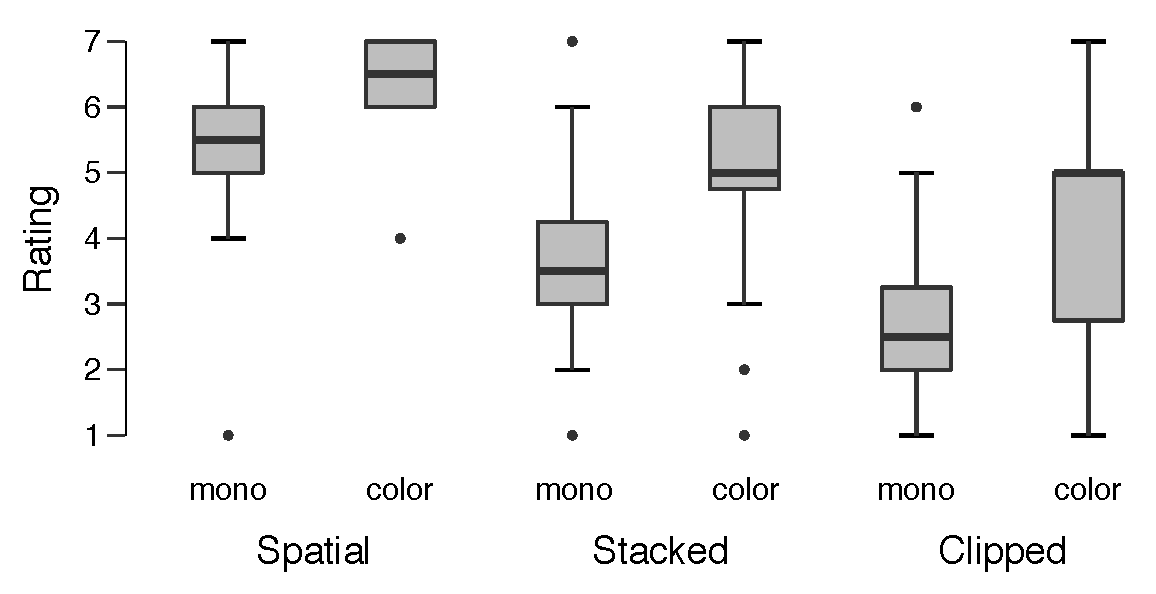
\includegraphics{post-color.pdf}
  \caption{Post-experiment ratings for different experiment types, \emph{Colored} and \emph{Monochrome}}
  \label{fig:post-color}
\end{figure}

The results mirror the other quantitative and qualitative outcomes, in that \emph{Spatial} and \emph{Colored} conditions were rated most highly. An individual one-way \textsc{anova} ($F\alpha = .05$) on the dependent variable rating shows a significant main effect from interface type ($F(2,114) = 30.55, p < .001$) and color ($F(1,114) = 23.19, p < .001$). A Tukey post-hoc test revealed that participants preferred \emph{Spatial} to both \emph{Stacked} ($p < .001$) and \emph{Clipped} ($p < .001$). It also shows that they preferred \emph{Colored} to \emph{Monochrome} ($p < .001$).

However, unlike the quantitative results, these results also show significant differences between \emph{Stacked} and \emph{Clipped}. In the same analysis we also found a significant preference for \emph{Stacked} over \emph{Clipped} ($p = .015$). This shows that participants perceived \emph{Stacked} and \emph{Clipped} differently, despite the fact that there was no significant difference in performance in our experiment.

\subsection{Participant Comments}
The comments we got from participants, both verbally during the experiment, and in the comments field on our post-experiment questionnaire, match our other findings for the most part. The most prevalent comment was that color made it much easier to find items because it narrowed down the search to only icons of the right color. This was mentioned by almost all partcicipants, though one participant expressed finding it confusing in \emph{Spatial} conditions.

\begin{quote}
  \emph{``Color helps find icons easily (even if you don't remember the location). Black/White is difficult to find.''}

  - participant 17
\end{quote}

Many participants also expressed a preference for \emph{Spatial} conditions, stating that they found it faster and easier to find items by looking around rather than scrolling a list.

Several participants also commented on their preference for \emph{Stacked} over \emph{Clipped}. This is consistent with the results from the Likert scale ratings, which also show a preference for \emph{Stacked}.
Multiple comments also mentioned being particularly annoyed by large \emph{Clipped} conditions, because the position in the list was not visible.

\begin{quote}
  \emph{``Clipped gives no indication where in the list I am (at 20\% or at 80\%).''}

  - participant 9
\end{quote}

One participant mentioned feeling like they were equally efficient with \emph{Clipped} compared to \emph{Stacked}, but \emph{Clipped} required more mental work because they had to rely entirely on their memory.

A few participants had problems with clicking items in scrolling conditions (\emph{Clipped} and \emph{Stacked}), which they mentioned both verbally and in comments. They were all able to complete the tasks, but it may have had a small impact on their performance in these conditions.

Several participants also mentioned feeling like \emph{Stacked} conditions were laggy and unresponsive compared to \emph{Clipped}. This may also have had an impact on their task performance. Interestingly, this did not seem to impact their preference for \emph{Stacked} over \emph{Clipped}. This may be connected to the fact that they liked how it looked (\emph{``Stacked looks more cool''} - participant 11), and the aforementioned sense of position in the list that \emph{Stacked} provides.

\begin{quote}
  \emph{``Clipped scrolls more smoothly than Stacked.''}

  - participant 13
\end{quote}

%----------------------------------------------------------------------------------------
%	DISCUSSION
%----------------------------------------------------------------------------------------

\chapter{Discussion}
\label{ch:discussion}

Our results show that spatial interfaces have the potential to make \textsc{vr} interfaces more efficient and pleasurable to navigate. \emph{Spatial} conditions were outperforming other conditions in both the quantitative and qualitative parts of our study. This confirms our initial assumptions, and shows the potential of using 3D space more fully in \textsc{vr} interfaces. Though we did not find any significant performance advantage in \emph{Stacked} over \emph{Clipped}, the fact that participants preferred it and mentioned being able to have a better sense of position within the list does mean that this interface type could potentially be promising, and should be explored further.

\section{Limitations}
Due to performance problems with our implementation, \emph{Stacked} conditions were laggier than \emph{Clipped} ones, rendering at lower frame rates and in some cases dropping frames aggressively. This happened to different degrees for different participants. It is hard to estimate the impact this had on the results, but it should be taken into account when discussing them. It is unlikely that a more performant implementation would have changed the results so drastically in favor of \emph{Stacked} that the difference would have been significant.

Another flaw in our implementation was that scrolling and clicking were done using the same controller button (the right hand trigger). We chose this interaction because we wanted it to be easy to get started with by mimicking the one-finger interaction on touch screens that we assumed all participants would be familiar with. Holding the trigger and moving it further than a certain threshold from the original position would scroll, releasing it without moving it would click. This mechanic worked well for most of our participants, but for a few of them it was difficult to click without moving the controller past the threshold. This meant that they would have to try clicking an icon several times before being able to select it, because they moved the controller too much before releasing and triggered a scroll instead of a click. This got better after the first few conditions, as participants learned to click more quickly and move the controller less. It is therefore unlikely that it impacted the results significantly.

\section{Future Work}
All the interfaces in our experiment had a spatial model. The difference between \emph{Clipped} and the other two conditions is that the spatial model is implicit. Just like on screens, elements that are not currently visible still exist in the user's mental model of the interface, they are just not currently visible. This may be part of the reason why we did not find a significant difference in performance between \emph{Stacked} and \emph{Clipped}. It would therefore be interesting to add interfaces with no spatial model (e.g. a paginated list with no animations) to the experiment. The difficulty in this case would be that the interactions could not be the same (scrolling is spatial by definition), which would make them harder to compare. However, given that pagination with non-spatial page transitions is a common navigation pattern in current-generation \textsc{vr} interfaces, it would be a very relevant comparison.

Another area that could be further explored is different spatial arrangements for items, like our \emph{Stacked} condition. We found that users liked it, but some mentioned that they could not see the elements very well from the front, which negates part of the benefit of this layout. Different layouts, like stacking cards on top and bottom instead of behind the list, could be explored in order to address this problem.

In order to have more context on people's scanning and navigation techniques, it would be interesting to run a similar study while tracking participants' eye movements \cite{card1984visual}. This could also help to understand the influence of color more clearly, as most participants mentioned that they found it helpful, while a few expressed that they found it distracting.

All of our participants had relatively little experience with \textsc{vr}. They used our interfaces for the first time during the experiment, and though we did have a set of tutorials introducing them to the interfaces, the novelty of it all was likely a factor in how participants performed in the experiments. It would therefore be interesting to perform a more long-term study, where participants use interfaces multiple times over a longer period. In order to understand whether the performance difference between \emph{Spatial} and the other conditions changes over time, as participants get more comfortable with the more interaction-heavy \emph{Stacked} and \emph{Clipped} conditions.


%----------------------------------------------------------------------------------------
%	CONCLUSION
%----------------------------------------------------------------------------------------

\chapter{Conclusion}
\label{ch:conclusion}

When a new medium emerges, it tends to emulate the constraints and idiosyncrasies of previous mediums at first. For example, early web pages were modeled after printed media, and therefore did not really make use of the new possibilities that screens afforded over print (e.g. dynamic, responsive layouts). As a medium matures, creators learn to use it more effectively, and it comes into its own as a separate medium rather than an extension of existing media. As Virtual and Augmented Reality technology advances and moves closer to the mainstream, we will likely see it undergo this transition as well.

Currently, \textsc{vr} interfaces are emulating traditional 2D interfaces for the most part. As the technology improves and designers become more familiar with the medium, they will increasingly want to make use of the fact that users can move their bodies in 3D space as part of their interactions with interfaces. This is the inherent advantage of \textsc{vr} compared to screen-based 2D interfaces, and it is why we believe that spatial interfaces are a very promising research area.

In this thesis we explored different types of spatial interfaces in Virtual Reality. We surveyed the relevant literature, the most common interaction techniques, and the current state of the technology. We then built a number of prototypes that explore different approaches to spatial \textsc{vr} interfaces, and conducted a study comparing them to a simple clipped list. The results show that spatial interfaces can help make interfaces more efficient and pleasurable to use, but it is dependent on the approach. We also found that even when there is no measurable performance difference, people preferred interfaces with an explicitly visible spatial model over ones that hide it. These results are encouraging, but further experimentation will be necessary to develop robust, scalable interface patterns for organizing information spatially. The dynamic nature of \textsc{vr} as a medium enables a myriad of new ways to display, structure, and navigate information that are yet unexplored.


%----------------------------------------------------------------------------------------

\backmatter

%----------------------------------------------------------------------------------------
%	BIBLIOGRAPHY
%----------------------------------------------------------------------------------------

\bibliography{bibliography} % Use the bibliography.bib file for the bibliography
\bibliographystyle{plainnat} % Use the plainnat style of referencing

%----------------------------------------------------------------------------------------

% \printindex % Print the index at the very end of the document

\end{document}
